%% ICN submission manuscript — compiled with XeLaTeX.
%% Author affiliations marked \emph{[...]} are placeholders to be completed.
\documentclass[10.5pt,compsoc,winfonts]{ICN}
\usepackage{fontspec}
\usepackage{graphicx}
\usepackage{booktabs}
\usepackage{multirow}
\usepackage{array}
\usepackage{longtable}
\usepackage[noadjust]{cite}
\usepackage{amsmath,amssymb}
\usepackage{float}
\usepackage{url}
\linespread{1.2}

\setmainfont{Carlito}[Ligatures=TeX]
\defaultfontfeatures{Ligatures=TeX}
\newcommand{\bta}{\fontspec{InriaSans-Bold.ttf}}
\newcommand{\bbb}{\fontspec{InriaSans-Light.ttf}}
\renewcommand\figurename{Fig.~}
\makeatletter
\renewcommand{\doi}[1]{\gdef\icn@doi{}}
\makeatother
\newcommand{\upcite}[1]{\cite{#1}}

\begin{document}

\title{Is Wireless Security Ready for the AI Era? A Scoping Review of 130 Studies, 2020–2026}

\firstheadname{Is Wireless Security Ready for the AI Era?}
\firstfootname{}
\headevenname{Is Wireless Security Ready for the AI Era?}
\headoddname{H.~T.~Siddiquee and M.~A.~M.~Fahim}

\author{\begin{tabular}{c}
Hussain Touhid Siddiquee$^{1*}$ and Md. Abul Malek Fahim$^{1}$\\
{\small $^{1}$Department of Computer Science and Engineering, \emph{[University]}, \emph{[City]}, \emph{[Postcode]}, Bangladesh}\\
{\small $^{*}$E-mail: touhidsiddiqueeraj@gmail.com}
\end{tabular}}

\abstract{Wireless links broadcast by physics, so the radio link is where AI-enabled
interception, spoofing and jamming land. This scoping review charts 130 studies published
2020–2026 that apply machine learning to wireless-link security or attack it, drawn from a
seeded search and two Crossref/arXiv runs and screened for radio population, security link, AI
involvement and evaluable evidence. Defenses dominate (84) over threats (30) and dual-track work
(7), while deep supervised learning (45) only narrowly leads adversarial machine learning (40).
Radio-frequency fingerprinting is the dominant function (69 of 121 core studies, 57.0\%),
artifact release remains rare (4, 3.3\%), and closed-loop attack–defense evaluation reaches at
least 14 studies (11.6\%). A blinded re-coding of 30 records gives good agreement for composition
items ($\kappa$ 0.68–0.84) but poor agreement for readiness items ($\kappa$ 0.11–0.39), so
readiness findings are directions, not magnitudes. On current evidence the literature does not
demonstrate wireless security ready for the AI era.}

\doi{}\par
\keyword{Wireless security; physical-layer security; radio-frequency fingerprinting; adversarial
machine learning; jamming; federated learning privacy; post-quantum migration; scoping review}

\maketitle\pagestyle{icnheadings}

\section{Introduction}
\label{sec:intro}
\subsection{The radio link under AI pressure}
Wireless links broadcast by physics: every transmission is receivable by anyone in range, which makes the radio link the natural attack surface for interception, impersonation, and jamming. The classical answer—encryption, authentication and key agreement (AKA), and physical-layer techniques—now faces three simultaneous strains. First, software-defined radios put laboratory-grade interception and transmission in every adversary's hands. Second, machine learning turns raw captures into fingerprints, keys, and exploits automatically, without hand-built demodulators. Third, autonomous systems (drones, vehicles, swarms, IoT/edge fleets) need authentication under real-time deadlines, over-the-air updates, and multi-agent trust—requirements the literature rarely addresses together. The question this review asks is whether the radio-link security literature has kept pace with the adversary it has itself equipped.

\subsection{How AI entered wireless security}
AI entered through authentication. Deep networks learned RF fingerprints from raw I/Q, outperforming hand-crafted features, and physical-layer key generation promised lightweight secrets from channel reciprocity without public-key infrastructure. The adversarial turn followed quickly: white-box FGSM/PGD perturbations and black-box universal perturbations (81.7\% success with almost no victim knowledge) break RFFI classifiers on real LoRa captures \upcite{T03}; reinforcement-learned impersonation needs only binary accept/reject feedback for $>$90\% penetration \upcite{T18} (an adversarial-ML attack—the defense-side DRL family counts control methods only, so Fig.~\ref{fig:methodtrack} shows no DRL threat rows); GAN-spoofed signals pass PHY authentication at 76\% \upcite{T09}. Two results reset expectations for the field: far-field deep-learning side-channel recovery of BLE AES-128 at 15~m from fewer than 400 traces \upcite{T01}, and Magmaw \upcite{T30} (NDSS'25)—protocol- and modality-agnostic universal perturbations, SDR-demonstrated at noise-level power, surviving adversarial training, subtraction, detection, and oracle defenses, including against an encrypted image channel. Authentication learned from waveforms, it turned out, could be unlearned by waveforms. Fig.~\ref{fig:milestones} places these turning points on a timeline: with two exceptions (a 2022 ensemble defense and a 2025 proactive-authentication defense), every milestone is an attack (milestones author-selected to mark field turns, not sampled).
\begin{figure*}[tbp]
\centering
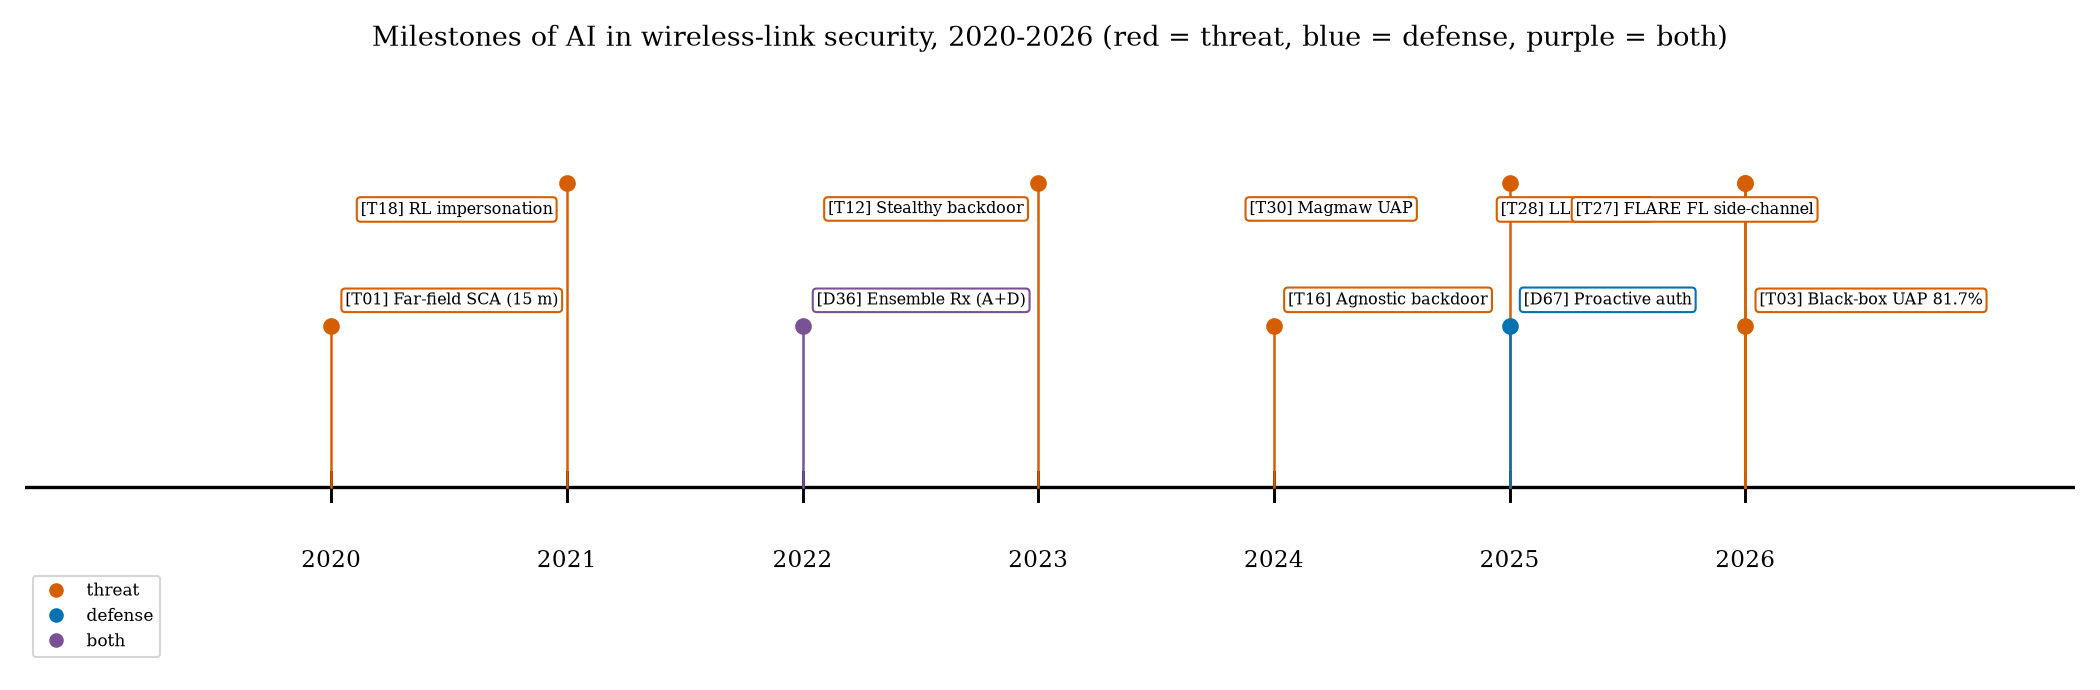
\includegraphics[width=17.0cm]{figures/FigC_milestones.png}
\caption{Milestones of AI in wireless-link security, 2020–2026. Red markers are threats, blue defenses, purple joint attack-plus-defense work.}
\label{fig:milestones}
\end{figure*}

\subsection{Existing reviews and the literature gap}
The review literature has grown alongside the applications, but it is fragmented along the same axes as the primary studies. Function-specific surveys cover RF fingerprinting \upcite{B03}; method-specific ones follow adversarial ML \upcite{B07}; the closest cross-functional account is a physical-layer-authentication survey for the ML era \upcite{B02}. Table~\ref{tab:priors} compares their scope and method against this review. What is largely missing is a cross-functional, quantitative account of the field's trajectory: which AI method families are actually being used for which security functions, on which data, validated how, and how that picture has shifted over 2020–2026. This gap matters because the field's self-image drives its research allocation. If most published authenticators are validated on closed-set, single-receiver, static-channel benchmarks, the community's sense of progress is calibrated to a regime that differs sharply from deployment under adaptive adversaries. Answering such questions requires a corpus-level, cross-functional account rather than another narrative synthesis of one function. This article therefore reports a structured scoping review, conducted and reported per the PRISMA-ScR extension, of machine learning applied to wireless-link security over 2020–2026.

\begin{table*}[tbp]
\centering
\footnotesize
\caption{Prior surveys closest to this review: scope, method, and what differs here.}
\label{tab:priors}
\begin{tabular}{@{}l p{3.6cm} p{2.6cm} p{5.2cm}@{}}
\toprule
Survey & Scope & Method & This review instead \\
\midrule
{\upcite{B03}} Jagannath 2022 & RFFI only & Narrative & 8 functions quantified jointly \\
{\upcite{B07}} Adesina 2023 & Adversarial wireless ML & Narrative & Plus defenses, validation grade, trends \\
{\upcite{B02}} Hoang 2024 & PLA/auth in ML era & Narrative & Plus threats, readiness scores, checklist \\
\bottomrule
\end{tabular}
\end{table*}

\subsection{Contribution of this paper}
This paper makes four contributions. First, it assembles a verified corpus of 121 core studies (2020–2026) on AI in wireless-link security broadly construed—authentication and RF fingerprinting, key generation, secure communications/anti-jamming, protocol and traffic analysis where the classifier is the security boundary, and federated privacy—plus 9 post-quantum-migration studies kept in a separate contextual stratum (130 records total). Every record carries a resolvable identifier verified against publisher metadata; two same-team companion pairs are counted as distinct records under a drop-one-pair sensitivity check, and one conference-to-journal extension was deduplicated (\S\ref{sec:methods}). Second, it develops a two-axis classification framework, security function $\times$ AI method family, extended with track, data-source, validation-practice, and readiness fields, and applies it uniformly to all 130 papers. Third, it quantifies the field's six-year evolution across functions, methods, data, and validation (\S\ref{sec:corpus}), tracing the shift from deep supervised fingerprinting through adversarial ML to DRL anti-jamming, federated privacy, and early LLM-assisted analysis. Fourth, it reviews function by function what the corpus actually demonstrates (\S\S\ref{sec:threat}–\ref{sec:pqc}), analyzes the cross-cutting threat–defense asymmetry (\S\ref{sec:cross}), and distills the resulting gaps into a research agenda and a twelve-item reporting checklist (\S\ref{sec:gaps}).
Fig.~\ref{fig:heatmap} previews the analysis, mapping the corpus across security functions and method families: the field's center of gravity sits squarely in the RFFI $\times$ (adversarial $+$ deep-supervised) complex, key generation is a simulation-heavy island, and LLM-assisted work is only now appearing. The remainder of the paper is organized as follows. \S\ref{sec:methods} details the review methodology. \S\ref{sec:corpus} presents the corpus overview and bibliometric analysis. \S\S\ref{sec:threat}–\ref{sec:pqc} review threats, defenses, and the quantum-era context. \S\ref{sec:cross} examines cross-cutting directions. \S\ref{sec:gaps} formulates gaps and the checklist. \S\ref{sec:conclusion} concludes.

\section{Method}
\label{sec:methods}
\subsection{Scope and objective}
The objective is to characterize the state and evolution of AI applied to radio-link security. The scope covers 2020-01-01–2026-10-11 and includes authentication/RF fingerprinting (including localization-fingerprint attacks where a geofence bypass breaks an authorization boundary), key generation/distribution/exchange/management, anti-jamming/secure communications, protocol/traffic/signal analysis where the classifier is the security boundary, side-channel analysis, federated privacy, and learned primitives—each crossed with AI as attacker tool, defender tool, or learned primitive. Readiness gaps for autonomous systems (drones, vehicles, swarms, IoT/edge) form the second axis of the review. Post-quantum migration is treated as a separate contextual stratum (9 studies, several of which meet neither the AI-link nor the radio-link criterion on their own and are retained as context only) and is never pooled with AI claims. No in-corpus paper joins an AI-driven attack with a post-quantum implementation over a radio link; this absence is recorded as a scoping result, with the caveat that the stratum was assembled without an AI-linkage requirement, so it describes this corpus rather than the field. The title question—is wireless security ready for the AI era?—is answered in \S\ref{sec:conclusion}.

\subsection{Literature search strategy}
The search combined three paths—programmatic retrieval, expert-seeded web rounds, and a database path—with the database path executed on the OpenAlex index because no institutional access to Scopus, IEEE Xplore, or Web of Science was available. Collection stopped after the seeded rounds, the two OpenAlex runs, and an adjudication pass; no formal stopping rule was applied. The programmatic pool of 241 records was held unscreened as backup, and the programmatic path contributed zero included records, so triangulation rests on the seeded and database paths. Path A (programmatic): Crossref REST API, 16 topical queries (rows=100, date/type filtered) plus arXiv API, 10 queries (max 50) $\rightarrow$ 1,945 unique records after DOI/arXiv-ID deduplication (1,555 Crossref $+$ 390 arXiv; \texttt{records.json}). Path B (expert-seeded): 29 structured open-web search rounds ($\sim$290 records, fully logged in \texttt{run\_log.md}) $\rightarrow$ 126 unique candidates by paper ID after deduplication (109 includes $+$ 12 background $+$ 4 backup $+$ 1 exclusion). Path C (database): 10 topical queries against the OpenAlex index (no subscription required), 894 hits deduplicated against Paths A–B to 662 new records, title-gated to 130 candidates (\texttt{code/openalex\_run.py}, \texttt{code/openalex\_gate.py}).

Two properties of this design shape how its yields should be read. First, Crossref is a metadata registry rather than a discovery engine like Scopus or Web of Science, and topical recall for this IEEE/ACM-heavy, terminology-variant literature is $\sim$50\% by token overlap—which is why the design triangulates across sources rather than relying on any single one. OpenAlex, which indexes the same publishers, substitutes for the pending subscription-database runs and satisfies database triangulation in part; full multi-registry triangulation remains future work. Its 10-query run surfaced 14 eligible papers missed by 29 seeded rounds plus 26 API queries, reported as evidence about search-recall limits rather than as a census. Second, the seeded path inherits expert-search bias toward notable and recent work; trend statements therefore describe this verified, English-language sample rather than the field in the aggregate.

\subsection{Screening and selection procedure}
The study-selection funnel is shown in Fig.~\ref{fig:flow}. From 1,945 deduplicated programmatic records, a title-level relevance gate requiring wireless, crypto/authenticity, and AI terminology retained 241 records (\texttt{gated.json}). These extension-pool records are released with their disposition (overlap with the seeded set or held for future screening) and were not merged silently into the evidence base, which rests on fully screened paths only.

The seeded path went from 126 unique candidates, screened against a validity floor (V1 peer-reviewed, in range, and retrievable; V2 evaluable evidence; V3 traceable claims), to 109 included records, 12 background survey-only landmarks, 4 backup needs-check rows held for later screening, and 1 title-gate exclusion (an EAP-AKA scheme with no AI link). The first database run went from 894 hits to 662 unseen records, title-gated to 130 candidates; abstract-level screening produced 14 included records, 2 background entries (a systematic O-RAN analysis and a conceptual quantum-ML plan, neither with a primary mechanism) and 1 exclusion (no cryptographic link), the remainder being out-of-scope surveys, non-radio, or intrusion-detection-only work. A second database run went from 994 hits to 743 post-deduplication, title-gated to 136, and produced 12 included records plus 8 exclusions with logged reasons.

An adjudication pass then applied scope and deduplication cuts to the merged pool: one record was subsumed by a later version of the same work, one carried no machine-learning content, one no cryptographic link, and one no radio link, while one moved to background under the sensing rule; two further records \upcite{T05,T14} were reclassified as dual-track under a single stated rule. The final corpus is 130 included studies (121 core: 84 defense, 30 threat, 7 both, plus 9 post-quantum context), 15 background, 4 backup, and 14 excluded.

Full-text curation of the 30 arXiv-sourced rows upgraded readiness scores where body text confirmed testbeds, threat models, costs, or artifacts (\texttt{fulltext\_reads.md}). A reconciliation pass then aligned R2 to the validation mapping (\S\ref{sec:methods}); it moved track R2 means upward by up to about 0.6 (dual $+$0.57) while preserving their order, and neither pass overturned the abstract-level picture. Three venue-resolution rounds subsequently confirmed 28 of the newly merged rows as published, each with a resolved DOI (\texttt{found\_papers.csv}).

The final corpus carries 19 preprints (14.6\%): 14 venue-unconfirmed arXiv-only entries, 2 presented-or-preliminary rows, 1 submitted row (a stated target conference inconsistent with its posting date, held unconfirmed), and 2 author-claimed rows without a proceedings record. No entry changed status without a logged resolution; the individual dispositions are listed in Tables~\ref{tab:corpus} and~\ref{tab:corpusb} and in the released dataset. The rerun delta was dominated by the previously rate-limited federated-learning query, a coverage artifact rather than one-day field growth: its 7 wireless-FL-privacy additions nearly triple the federated-privacy function (4 $\rightarrow$ 11), reported as a coverage correction in \S\ref{sec:corpus}, not as field growth.

\begin{figure*}[tbp]
\centering
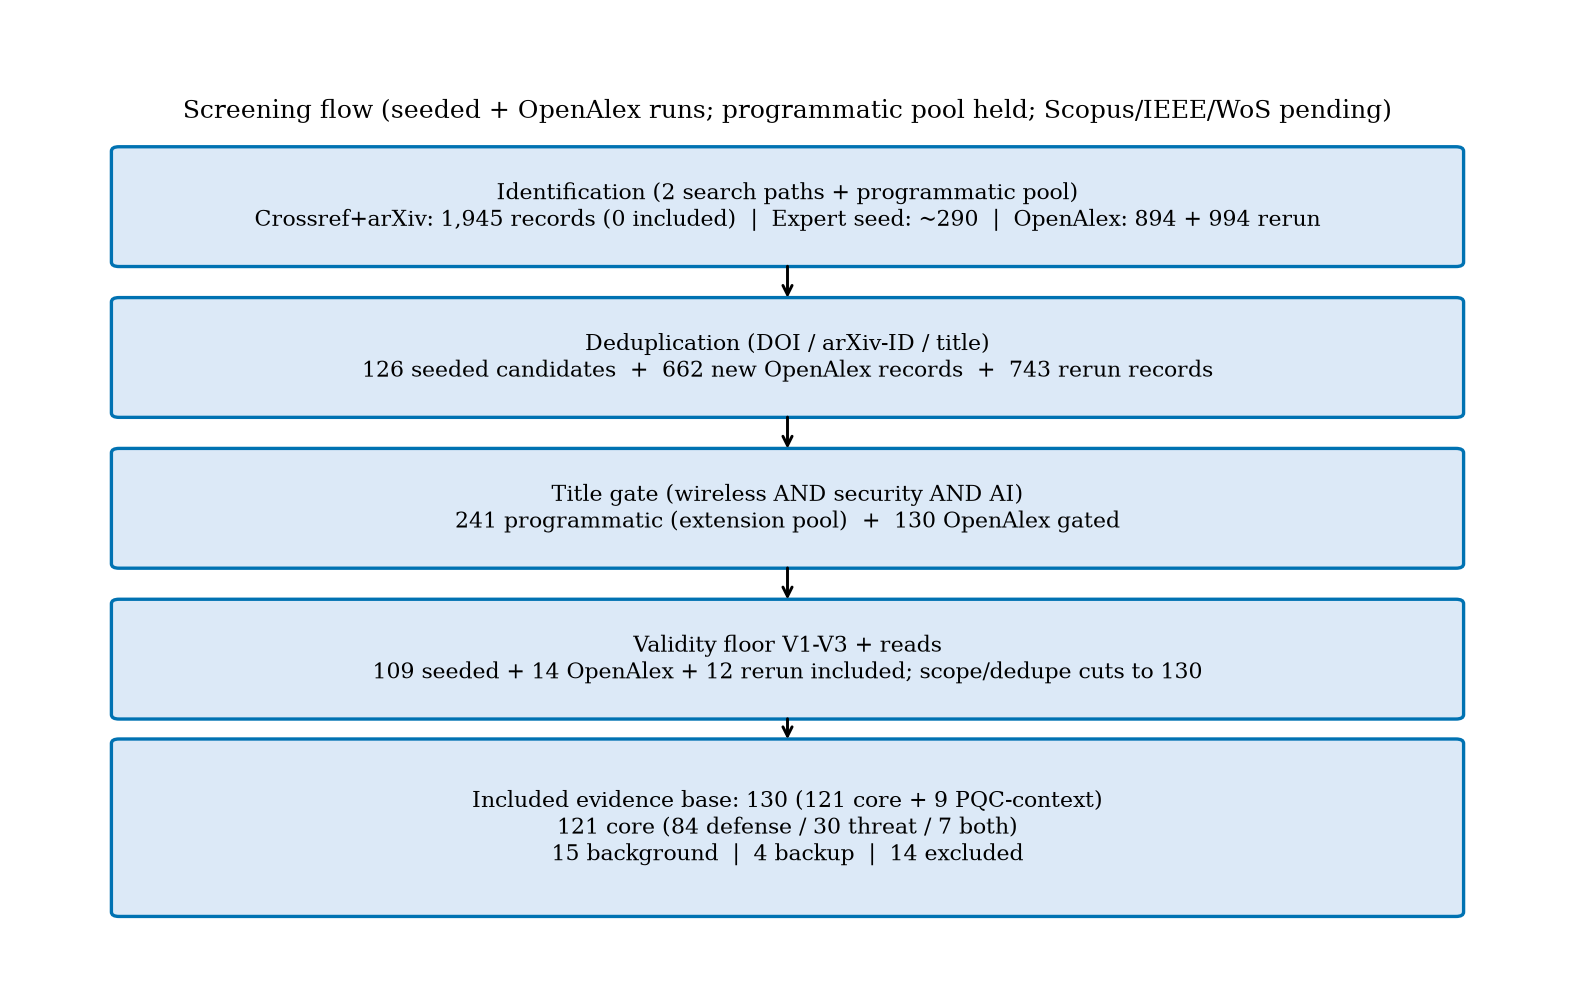
\includegraphics[width=13.3cm]{figures/Fig1_screening_flow.png}
\caption{Study-selection flowchart. Programmatic records were retrieved from the Crossref and arXiv APIs (Path A, 241 gated extension-pool records released with disposition, not merged silently), OpenAlex database hits were deduplicated against them and title-gated (Path C), the expert-seeded path and two OpenAlex database runs were screened against the validity floor, an adjudication pass applied scope and dedupe cuts before the corpus froze at 130 studies (105 seeded $+$ 13 OpenAlex $+$ 12 rerun). Every record carries a verified resolvable identifier (see \S\ref{sec:intro}).}
\label{fig:flow}
\end{figure*}

\subsection{Inclusion and exclusion criteria}
Table~\ref{tab:criteria} summarizes the criteria. Inclusion required: (i) a radio-link/wireless population; (ii) a security link (broad wireless-ML-security scope per \S\ref{sec:intro}: encryption, authentication including localization-fingerprint attacks where a geofence bypass breaks an authorization boundary, key exchange/management/generation, physical-layer security, anti-jamming/secure communications, signal/traffic analysis where the classifier is the security boundary, side-channel analysis, federated privacy); (iii) AI involvement; (iv) dated 2020–2026, English, retrievable; (v) evaluable evidence (experiment, testbed, simulation, proof, cryptanalysis); (vi) a peer-reviewed venue or reputable arXiv preprint (ID, version, and access date; published supersedes; preprints $\le$40\%—observed 14.6\%). Exclusion: not wireless; no security link; no AI link; survey/opinion without primary mechanism (background only); pre-2020; non-English; retracted; unretrievable; no evaluable evidence; preprint without evaluation; and duplicate (one same-team conference-to-journal extension deduplicated, while two same-team companion pairs \upcite{D55,T15}; \upcite{D20,T20} were counted as distinct records with disclosure, each under a drop-one-pair sensitivity check).

The boundary rulings were applied consistently and are logged in full in the released screening log. Cellular fuzzing without machine-learning content is excluded for failing AI involvement; Wi-Fi localization-fingerprint attacks are included where a geofence bypass breaks an authorization boundary, rather than on a forgery-breaks-authentication claim; signal-classifier attacks are included where the classifier is the security boundary; IoT traffic-classifier attack-plus-defense work counts as dual-track protocol work. Wireless federated-learning privacy counts where the privacy guarantee is produced by channel properties (over-the-air superposition, channel-noise differential privacy)—a physical-layer mechanism—while generic federated-learning applications without a channel-produced guarantee are excluded. Acoustic and vibration side-channel analysis of post-quantum schemes fails the radio-link population; Wi-Fi sensing without a security link moved to background; 5G regression-robustness work without a security boundary is excluded. The venue rule was applied in both directions: author-claimed venues without a proceedings record were coded preprint, while author claims confirmed by a publisher record stayed peer-reviewed.

All screening, eligibility coding, and charting were performed by the review team against the stated rubric, and the complete coded dataset is released as \texttt{dataset\_papers.csv} so independent researchers can check, correct, or extend any record. Every record carries a resolvable identifier checked against Crossref, arXiv, ACM, or USENIX; record-level corrections applied during verification (re-keyed venue attributions, two year corrections to published versions, two preprint recodings) are logged in the released run log.

\begin{table*}[tbp]
\footnotesize
\centering
\caption{Inclusion and exclusion criteria applied during corpus screening.}
\label{tab:criteria}
\begin{tabular}{@{}p{2.2cm} p{5.5cm} p{6.0cm}@{}}
\toprule
Dimension & Included & Excluded \\
\midrule
Population & Radio-link/wireless systems & Wired-only, pure sensing without crypto link \\
Concept & Crypto primitive $+$ AI involvement & Missing either link \\
Document & Peer-reviewed $+$ reputable arXiv ($\le$40\%) & Surveys w/o mechanism, evidence-free preprints \\
Period & 2020–2026 & Pre-2020 \\
Verification & DOI/arXiv-ID resolved & Unresolvable, retracted, duplicate \\
Language & English & Non-English \\
\bottomrule
\end{tabular}
\end{table*}

\subsection{Classification framework}
Each paper was classified along six fields. (1) Security function, 8 values: Authentication/RFFI, Key generation/distribution, Anti-jamming/secure comms, Protocol/traffic/cryptanalysis, PQC migration contextual, Federated/privacy-preserving FL, Learned primitives/crypto, Side-channel attack analysis. (2) AI method family: adversarial ML, deep supervised, PQC implementation, reinforcement/DRL, federated/private, traffic-analysis ML, LLM-assisted, defensive/robust ML, classical/Bayesian, optimization-based, dataset/benchmark, survey. (3) Track (threat 30 / defense 84 / both 7 / pqc-context 9), with \upcite{T05}/\upcite{T14} moved to dual-track under the develops-and-evaluates-both rule. (4) Primary data source. (5) Validation approach. (6) Readiness R1–R5, each scored 0–2 with N/A handling under an explicit rubric:
\begin{itemize}\setlength\itemsep{1pt}
\item R1 (all rows): 0 absent / 1 implicit / 2 explicit attacker capability $+$ assumptions.
\item R2 (all rows): 0 theory/proof/analysis without data evaluation / 1 controlled evaluation (simulation, reused datasets or traces, cross-domain protocols on collected data) / 2 author-conducted OTA/testbed demonstration or demonstrated real key recovery. As applied, simulation-only rows score 1 per this rubric, and the mapping is asserted programmatically over all 130 rows with one documented override (\upcite{T01}: standard-split validation with R2=2 for demonstrated over-the-air key recovery, without which the threat mean would read 1.50).
\item R3, reported for defense and learned-crypto/auth rows: 0 no cost / 1 latency OR energy $+$ hardware target / 2 both $+$ hardware target; on attack-only rows it applies only where an observable attacker cost is reported (6 rows, mention-level), otherwise coded 0, with fuller reported costs charted in \texttt{attacker\_cost}.
\item R4 (all rows): 0 neither / 1 code OR data / 2 both or artifact-evaluated.
\item R5, reported for defense and PQC-context rows: 0 none / 1 mentions 3GPP/IETF/NIST/ETSI / 2 evaluated against a profile; on attack-only rows it applies only where the paper names an affected standard (5 rows, mention-level), otherwise coded 0.
\end{itemize}
Rows without an observed signal are coded 0. Attack-side values are never pooled into defense-side claims: R3 means are reported over defense rows only (mean 0.19, median 0), and R5 over defense, dual, and PQC-context rows (means 0.07/0.14/0.56, medians 0/0/1); including the attack-side signals, the threat-track means are R3 0.20 / R5 0.17. Papers take a single dominant value per field, and coding was conservative throughout (abstract-level, except where full-text reads are logged in \texttt{fulltext\_reads.md}; the 32 unclear-source rows remain a stated limitation). Each paper additionally carries a venue channel—journal (65), conference/workshop (46), or preprint (19)—coded from confirmed venue strings for the channel analysis in \S\ref{sec:sensitivity}. Counts should be read as one documented coding, with the release of the complete dataset (\texttt{dataset\_papers.csv}) allowing independent checking, correction, or extension of any record; a glossary of frequently cited corpus IDs accompanies the archive (\texttt{data/glossary.md}).

\subsection{Coding reliability}
\label{sec:reliability}
A second coder, blind to the first coding, re-coded 30 of the 110 abstract-coded records from the
same abstract strings against the rubric above. The sample was drawn deterministically (12 threat,
5 dual-track, 4 post-quantum, 9 defense; all seven years; all three venue channels; two records
with an exercised attacker-cost value), and the frozen sample and a blank score sheet were
committed to the released repository before scoring, so the sample could not be tuned to the
result. Agreement is Cohen's $\kappa$ with 2,000-sample bootstrap intervals: quadratic weights for
the ordinal items, no weights for the nominal ones, and raw agreement only for artifact release,
which has no variance in this stratum.

Agreement is good for security function (0.84), venue channel (0.83), track (0.72), standards
signal (0.76) and method family (0.68), and poor for attacker-model explicitness (0.39), data
source (0.38), evaluation realism (0.29), validation approach (0.21) and cost signal (0.11)
(Table~\ref{tab:reliability}). The low values are not an artifact of chance correction:
unweighted $\kappa$, Krippendorff's $\alpha$ and Gwet's AC1 agree for four of the five, none
lifting them above 0.43; cost signal is a separate case, since 19 of 30 records sit at the floor
for both coders, which makes the item uninformative rather than contested. A clarification round
that rewrote only the five weak items, keeping the standards item unchanged as a control, did not
improve them (control unchanged at 0.76), so the residual disagreement lies in what abstracts
report rather than in rubric wording.

Two consequences follow for the rest of this article. Composition counts—function, track, method
family, venue—rest on agreement of 0.68–0.84 and are read as counts. Readiness comparisons rest
on agreement of 0.11–0.39; they are reported as directions and their quantities as bounds, and no
finding in this review turns on a fine-grained readiness contrast. Both score sheets, the frozen
sample, the codebook for the clarification round and the agreement script are released with the
corpus.

\begin{table*}[tbp]
\centering
\footnotesize
\caption{Inter-coder agreement over 30 blindly re-coded abstract-depth records, before
adjudication. Values are Cohen's $\kappa$; the nominal items carry no weights and are measured
once, while the five weak items and one control item were re-scored under a clarified codebook.}
\label{tab:reliability}
\begin{tabular}{@{}lcc l@{}}
\toprule
Item & $\kappa$ (round 1) & $\kappa$ (round 2) & Reading \\
\midrule
Security function      & 0.84 & —  & good \\
Venue channel          & 0.83 & —  & good \\
Standards signal (R5)  & 0.76 & 0.76 & good; control, unchanged \\
Track                  & 0.72 & —  & good \\
Method family          & 0.68 & —  & acceptable \\
Attacker model (R1)    & 0.39 & 0.38 & poor \\
Data source            & 0.38 & 0.38 & poor \\
Evaluation realism (R2)& 0.29 & 0.29 & poor \\
Validation approach    & 0.21 & 0.20 & poor \\
Cost signal (R3)       & 0.11 & 0.11 & uninformative, floor-coded \\
Artifact release (R4)  & —  & —  & no variance; raw agreement only \\
\bottomrule
\end{tabular}
\end{table*}

\subsection{Comparative synthesis approach}
Quantitatively, classification fields are aggregated into cross-tabulations—function by year, method by year, data, validation, readiness per track—that characterize the corpus as a sample (\S\ref{sec:corpus}). Every figure and count was generated programmatically from the released dataset (see \texttt{code/}; \texttt{check\_consistency.py} gates export on sums and caption n-values). Qualitatively, the review synthesizes each function critically: what each cluster assumes, demonstrates, and where its support is thin (\S\S\ref{sec:threat}–\ref{sec:cross}).

Four limitations of the methodology should be weighed. First, search coverage: open-web seeding favors notable work, and the two OpenAlex yields (14 then 12 eligible) are reported as recall evidence—the first run was incomplete, its federated-learning query hit rate limits, so the “14 papers missed by seeded search” indicate search limits rather than saturation; no formal stopping rule was applied (collection stopped after the rerun plus adjudication pass), the programmatic path contributed zero included records, and the programmatic pool is held as backup. Second, coding depth: title-gate screening can miss nonstandard terminology, 110 rows are coded from abstracts (including all 32 unclear-source rows, concentrated in paywalled journals at 23 of 32) and only 20 were body-read, and body reads only ever upgraded scores—so all R3–R5 rates are lower bounds by construction, and Table~\ref{tab:validation} mixes coding depths (full-text rows skew simulation-heavy, 5 of 20, relative to abstract-coded rows, 13 of 110); full R3–R5 body reads remain future work. Third, coding reliability: agreement was measured on 30 of the 110 abstract-coded records and is poor for five readiness items (\S\ref{sec:reliability}), so the remaining 80 abstract-coded rows and the 20 body-read rows rest on a single coding, and readiness comparisons are reported as directions rather than magnitudes. Fourth, scope of synthesis: preprint inclusion adds recency at the cost of version instability (frozen by identifier, version, and access date; 19 preprints, 14.6\%, sensitivity-checked), full multi-registry triangulation (Scopus/IEEE Xplore/Web of Science) remains pending with OpenAlex as the executed substitute, and no pooled effect sizes or significance tests are reported—metric heterogeneity (accuracy vs KGR vs secrecy rate vs attack-success rate) forbids pooling by design, so function $\times$ validation cross-tabulations are descriptive and the WIRELESS-AI-RC checklist is scored against the corpus descriptively (\S\ref{sec:gaps}). \S\ref{sec:corpus} should therefore be read as a structured sample, not a census—which is why this paper describes itself as a scoping review with bibliometric classification rather than a meta-analysis.

\section{Results}
\subsection{Corpus overview and six-year evolution}
\label{sec:corpus}
Two kinds of number appear in this section. Composition numbers—how many papers do
what, in which venue, with which method family—carry measured inter-coder agreement of
0.68–0.84 (\S\ref{sec:reliability}) and can be read as counts. Readiness numbers—attacker-model
explicitness, evaluation realism, cost, standards—carry agreement of 0.11–0.76, and the
weakest items bound rather than certify any level comparison. Where a quantity depends on a weak
item it is given as an upper bound or a range, and the underlying codings are released.
\subsubsection{Publication trend}
The corpus spans 2020–2026 with a rising but non-monotonic profile: 4 (2020), 17 (2021), 10 (2022), 21 (2023), 29 (2024), 36 (2025), 13 (2026 partial) (Fig.~\ref{fig:composition}). The 2021 bump is substantially a coverage effect: 5 of the 7 rerun-added FL-privacy papers date to 2021, without which the year reads 12. Excluding those 7 as a sensitivity check (N=123): defense R2 reads 1.32 instead of 1.27 while threat R2 is unchanged at 1.53, and simulation-only reads 16 instead of 18—the threat-realism lead, dual-track lowest realism, and RFFI dominance hold either way. Two caveats: the corpus is curated, so the curve partly reflects curation as well as field growth; and preprint share rises with recency, which is the velocity justification for their inclusion (\S\ref{sec:sensitivity}). With those caveats, the profile matches the field's post-2020 SDR-democratization and the 2024–2025 adversarial-ML surge. Sensitivity: dropping either duplicate-ID pair (\upcite{D55}/\upcite{T15} or \upcite{D20}/\upcite{T20}) moves yearly totals by at most one paper and leaves the acceleration pattern unchanged.

\begin{figure*}[tbp]
\centering
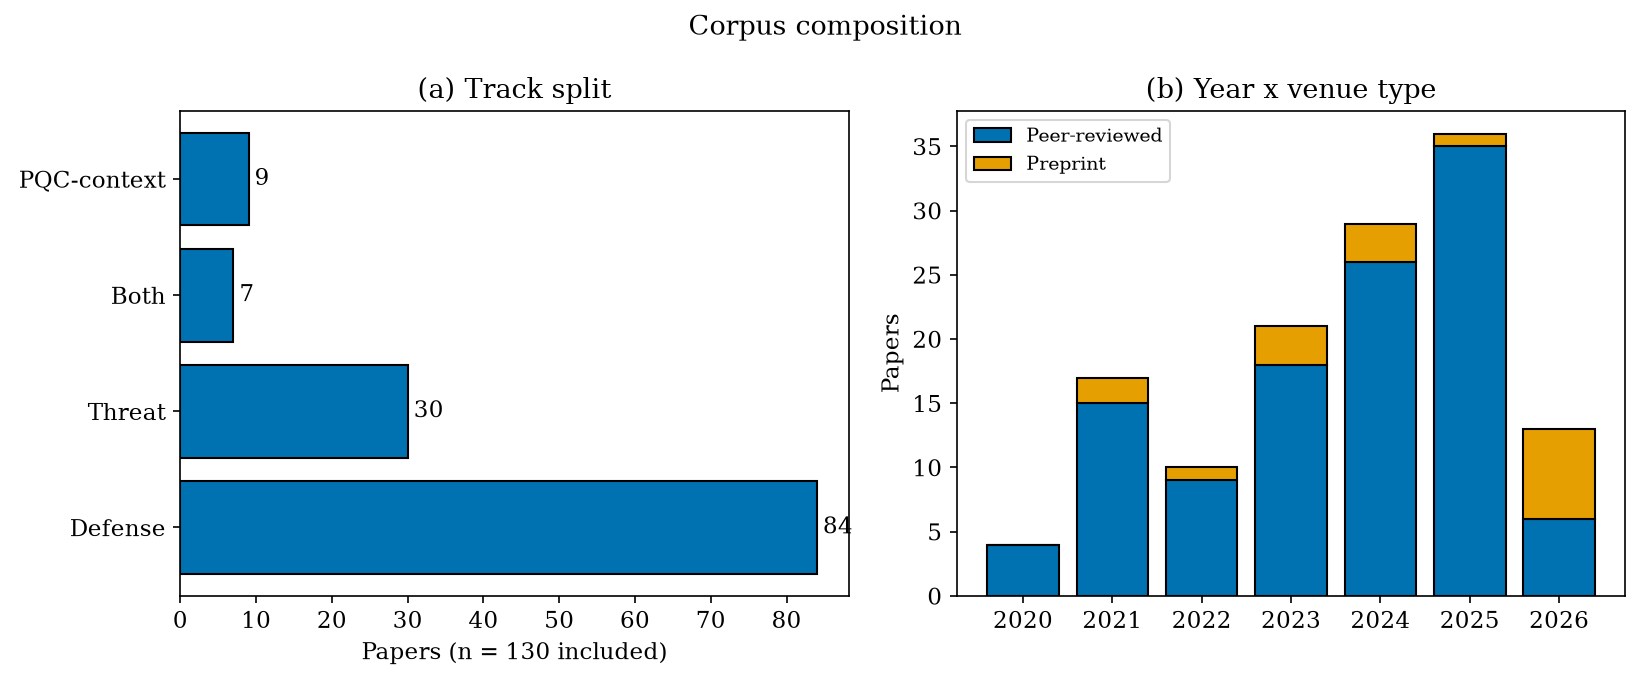
\includegraphics[width=14.0cm]{figures/Fig2_corpus_composition.png}
\caption{Corpus composition: (a) track split (n=130); (b) year $\times$ venue type. Preprint share rises with recency.}
\label{fig:composition}
\end{figure*}


\subsubsection{Method-family evolution}
Deep supervised learning leads with 45 papers against 40 adversarial ML (Table~\ref{tab:methods}), a five-paper margin that is not robust to corpus boundaries: a later merge added four deep-supervised RFFI papers while removing two adversarial ones, and the federated-privacy additions sit in neither family. Deep supervised work led in every year through 2023 (2–1 in 2020 through 9–7 in 2023); 2024 is adversarial's peak year (11 papers) but not a permanent lead change, and 2026 stands 3–4. Deep supervised totals 21 papers through end-2023, and only 33 of its 45 address RFFI, so “deep supervised fingerprinting” mislabels the family (remainder: key generation 8, side-channel 2, anti-jamming 1, protocol/traffic 1). Adversarial ML spans white-box, black-box UAP, GAN-spoofing, backdoors, and universal PHY perturbations, with the 2025–2026 wave adding self-supervised-target backdoors \upcite{T41}, over-the-air Wi-Fi attacks \upcite{T42}, and frequency-selective strikes \upcite{T44}. Reinforcement/DRL holds at 9, all defense-side (anti-jamming, UAV relay, secrecy-rate optimization). PQC implementation (9) concentrates 2024–2026. Federated/private learning climbs to 12—nearly tripled by the rerun coverage correction, reported as such rather than as field growth—traffic-analysis ML (2), a single LLM-assisted fuzzer (ConSeT \upcite{T28}, 2026), defensive/robust ML (2), dataset/benchmark contributions (2), survey/systematization (6), classical/Bayesian (1), and optimization-based (1) fill the long tail; protocol fuzzing/analysis leaves the taxonomy with \upcite{T07}'s exclusion. The sole classical/Bayesian paper sits under RFFI. The families are not mutually exclusive in practice; dominant-family coding understates mixing.

\begin{table*}[tbp]
\centering
\scriptsize
\setlength{\tabcolsep}{2pt}
\caption{Method families in the corpus: representative techniques, strengths, and limitations.}
\label{tab:methods}
\begin{tabular}{@{}>{\raggedright\arraybackslash}p{2.5cm} >{\raggedright\arraybackslash}p{0.9cm} >{\raggedright\arraybackslash}p{2.9cm} >{\raggedright\arraybackslash}p{2.9cm} >{\raggedright\arraybackslash}p{2.9cm}@{}}
\toprule
Method family & Papers & Techniques & Strengths & Limitations \\
\midrule
AdvML & 40 & FGSM/UAP, GAN-spoof, backdoor & Threat evidence; OTA-demo & Split 20 threat / 7 dual / 13 defense \\
DeepSup & 45 & CNN/RNN/Transf., open-set & Closed-set accuracy & Accuracy $\ne$ auth \\
PQC-impl & 9 & ML-KEM/ML-DSA, WKyber, LAKE & Onboard costs & Bandwidth blocks \\
DRL & 9 & Anti-jam power/relay & Adaptive control & Mixed grades (5 testbed); cost-silent \\
Fed/priv & 12 & DP-OTA-FL, robust aggregation & Privacy $+$ wireless-aware & Small scale; coverage-corrected \\
DataBench & 2 & Trace sets, open-set benchmarks & Reusable evidence & Rarely released \\
DefML & 2 & Robust training, unlearning & Adversary-aware training & Thin \\
TrafficML & 2 & Flow/classifier models & Deployed-boundary relevance & Evasion-prone \\
Survey & 6 & Reviews, maps & Maps field & No primary validation \\
Other & 3 & KNN/SVM, SCA/SDR, LLM fuzzing & Niche depth & Thin, scattered \\
\bottomrule
\end{tabular}
\end{table*}


Three observations qualify this trajectory. First, the families overlap in practice and dominant-family coding understates method mixing. Second, the adversarial rise is partly a response to the recognized brittleness of fingerprint classifiers under domain shift—but attack papers are, on average, evaluated no more stringently against adaptive defenses than defense papers are against adaptive attacks (\S\ref{sec:threat}), and no cited threat paper exploits domain shift as a standalone vector (\upcite{T40} documents consistent cross-device misclassification under domain shift and demonstrates its use as a backdoor for system intrusion on real-world experiments—attack surface with a demonstrated trigger, not a deployed exploit). Third, the LLM-assisted cluster is too small to represent a trend; its significance is that LLM-based baseband analysis is appearing at all.

\subsubsection{Application-area distribution}
Functionally the corpus is dominated by Authentication/RFFI: 69 of 121 core (57.0\%), followed by Anti-jamming/secure comms (14), Key generation/distribution (12), Federated/privacy FL (11), Protocol/traffic/cryptanalysis (10), PQC-context (9), Learned primitives (3), Side-channel analysis (2) (Fig.~\ref{fig:heatmap}, Table~\ref{tab:functions}). The center of gravity sits in RFFI $\times$ (adversarial 27 $+$ deep-supervised 33)—deep supervised now leads inside RFFI as well as overall. By contrast, learned primitives (3) are thin—telling, since these are where cryptographic consequences are most direct. Cutting the same data by track (Fig.~\ref{fig:methodtrack}) sharpens the asymmetry that \S\S\ref{sec:threat}–\ref{sec:defense} develop: adversarial ML splits 20 threat / 7 dual / 13 defense across tracks, deep supervised learning remains predominantly a defense instrument (42 defense vs 3 threat), and all reinforcement learning in the corpus sits on the defense side. Method-by-track figures pool dual-track papers with threat for readability; the text always gives the three-way split (for adversarial ML: 20 threat / 7 dual / 13 defense).
\begin{figure*}[tbp]
\centering
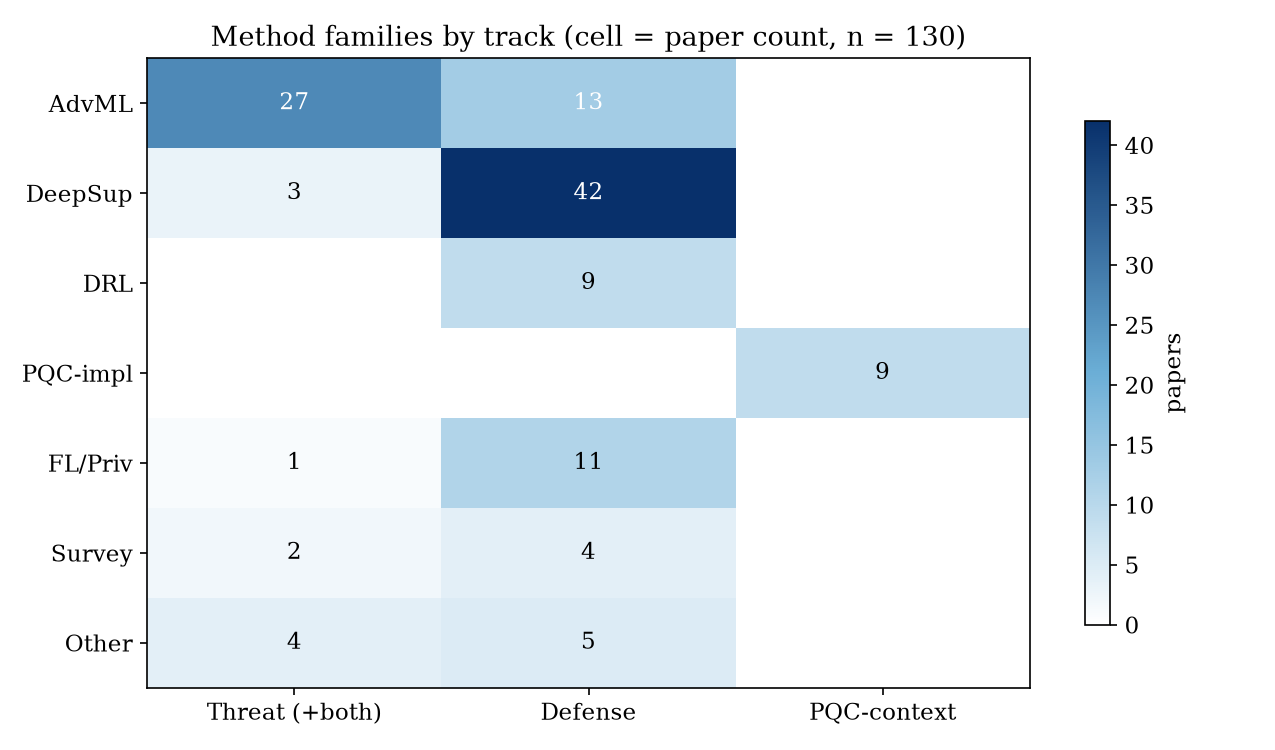
\includegraphics[width=10.8cm]{figures/FigB_method_by_track.png}
\caption{Method families by track. Adversarial ML attacks; deep supervised learning defends; reinforcement learning is defense-only in this corpus.}
\label{fig:methodtrack}
\end{figure*}

\begin{figure*}[tbp]
\centering
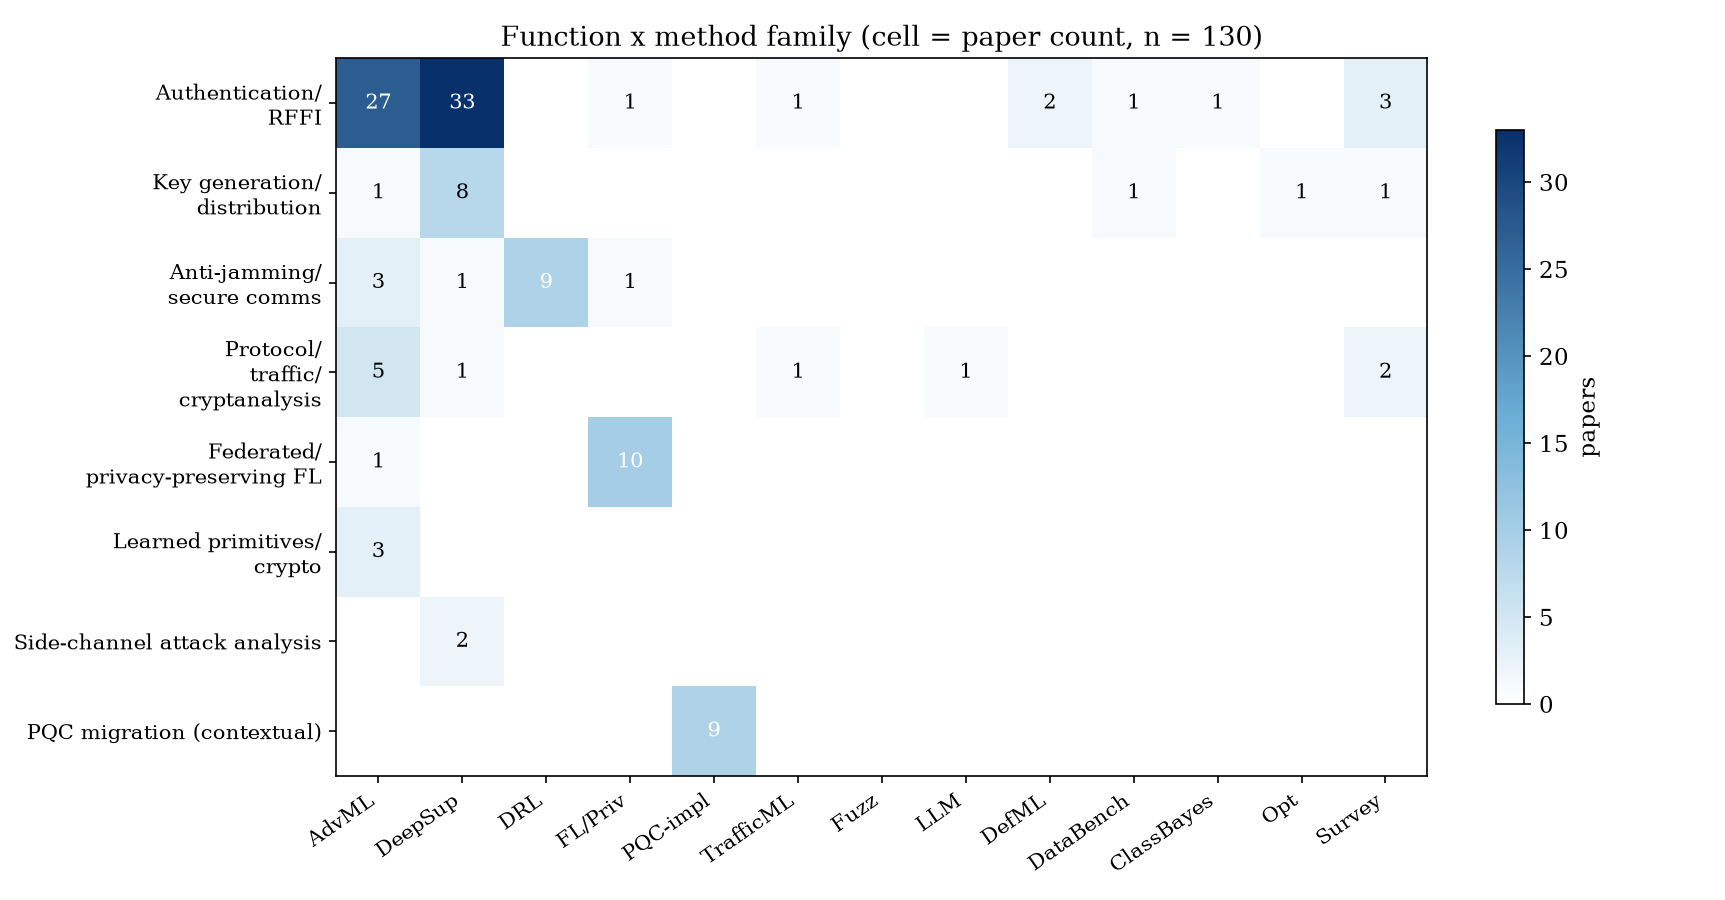
\includegraphics[width=14.6cm]{figures/Fig3_function_method_heatmap.png}
\caption{The corpus mapped across security functions and AI method families (n=130). Cell values are paper counts.}
\label{fig:heatmap}
\end{figure*}

\begin{table*}[tbp]
\footnotesize
\centering
\caption{Corpus composition: security function by publication year (130 papers). Machine-generated from the released dataset.}
\label{tab:functions}
\begin{tabular}{lrrrrrrrr}
\toprule
Function & '20 & '21 & '22 & '23 & '24 & '25 & '26 & Total \\
\midrule
Authentication/RFFI & 2 & 6 & 5 & 12 & 15 & 21 & 8 & 69 \\
Anti-jamming/secure comms & 0 & 0 & 2 & 3 & 6 & 3 & 0 & 14 \\
Key generation/distribution & 0 & 2 & 1 & 3 & 3 & 2 & 1 & 12 \\
Federated/privacy FL & 1 & 7 & 0 & 1 & 1 & 0 & 1 & 11 \\
Protocol/traffic/cryptanalysis & 0 & 0 & 1 & 2 & 2 & 3 & 2 & 10 \\
PQC migration (contextual) & 0 & 1 & 1 & 0 & 1 & 5 & 1 & 9 \\
Learned primitives & 0 & 1 & 0 & 0 & 1 & 1 & 0 & 3 \\
Side-channel analysis & 1 & 0 & 0 & 0 & 0 & 1 & 0 & 2 \\
Total & 4 & 17 & 10 & 21 & 29 & 36 & 13 & 130 \\
\bottomrule
\end{tabular}
\end{table*}

\subsubsection{Data landscape and validation practice}
Data sources are charted in Fig.~\ref{fig:data} (left) and Table~\ref{tab:data} (a data-source field, distinct from validation): testbed/OTA measurement 46, collected datasets/traces 26, simulation 20, analysis/benchmark 6, and 32 unclear from abstract. Validation practice (right panel): testbed/field demonstration 47 (36\%), cross-domain/generalization 26 (20\%), simulation-only 18 (14\%), standard split/unclear 35, and benchmark/analysis 4.

Crossing validation with track substantiates the section's headline (Fig.~\ref{fig:data}). Among threat papers (n=30), 16 are testbed/field demonstrations under the primary coding, 9 standard splits, 2 cross-domain, 2 simulation-only, and 1 benchmark—a measured plurality, not a norm. The testbed figure is an upper bound of roughly 10–16: the two codings found 6 and 4 such records among the 12 sampled attack records (\S\ref{sec:reliability}), with 8 threat data sources unclear from the abstract. Key generation carries the simulation-only mass (7 of 12 keygen papers simulation-only; defense sim-only 16 of 84—Table~\ref{tab:funcval}).

Readiness means per track (attack-only rows carry R3/R5 only where an observed attacker-cost or standards signal exists; no attack-side value is pooled into defense-side claims) are as follows: threat R1 1.70 / R2 1.53 / R3 0.20 / R5 0.17; defense R1 1.14 / R2 1.27 / R3 0.19 / R4 0.02 / R5 0.07; both (n=7) R1 1.86 / R2 1.14 (lowest realism); and PQC-context R3 1.11 / R5 0.56—the only stratum with real cost and standards numbers (ESP32 DTLS 313~ms, sub-12~kB Dilithium, Cortex-M4 cycles; FIPS 203/186, 3GPP, 802.11, O-RAN references). Medians are reported with the rubric in \S\ref{sec:methods}: R3 median 0 on defense rows; R5 medians 0 on defense and dual rows and 1 on PQC-context rows. Fig.~\ref{fig:readiness} plots the means by track (R1–R5 for all tracks; attack-side R3/R5 signals are mention-level). Table~\ref{tab:rdist} gives the underlying 0/1/2 count distributions (means are reported alongside, never alone), and Table~\ref{tab:ryear} shows readiness reporting by year: cost, artifact, and standards reporting stays flat while output multiplies, even as validation grade improves by share—volume and maturity do not move together.

\begin{table}[tbp]
\centering
\footnotesize
\caption{Readiness-score count distributions (0/1/2) over all 130 rows. R3/R5 zeros include attack-only rows without an observed attacker-cost or standards signal.}
\label{tab:rdist}
\begin{tabular}{@{}lccc@{}}
\toprule
Score & 0 & 1 & 2 \\
\midrule
R3 cost & 101 & 25 & 4 \\
R4 artifacts & 126 & 4 & 0 \\
R5 standards & 113 & 17 & 0 \\
\bottomrule
\end{tabular}
\end{table}

\begin{table*}[tbp]
\centering
\footnotesize
\caption{Readiness means by publication year (n in parens): cost/artifact/standards reporting stays flat while output grows.}
\label{tab:ryear}
\begin{tabular}{@{}lccccccc@{}}
\toprule
 & 2020 (4) & 2021 (17) & 2022 (10) & 2023 (21) & 2024 (29) & 2025 (36) & 2026 (13) \\
\midrule
R3 mean & 0.00 & 0.29 & 0.10 & 0.24 & 0.28 & 0.25 & 0.38 \\
R4 mean & 0.00 & 0.00 & 0.00 & 0.00 & 0.00 & 0.09 & 0.08 \\
R5 mean & 0.00 & 0.12 & 0.10 & 0.05 & 0.17 & 0.14 & 0.23 \\
\bottomrule
\end{tabular}
\end{table*}

\begin{table*}[tbp]
\footnotesize
\centering
\caption{Data sources recurring across the corpus.}
\label{tab:data}
\begin{tabular}{@{}>{\raggedright\arraybackslash}p{4.2cm} c >{\raggedright\arraybackslash}p{8.5cm}@{}}
\toprule
Data source & Papers & Typical use \\
\midrule
Testbed/OTA measurement & 46 & SDR captures, LoRa/Wi-Fi/UAV field demos \\
Collected datasets/traces & 26 & WiSig-style RFFI, RF-SCA trace sets \\
Simulation & 20 & Keygen channels, DRL jamming games, FL-privacy analysis \\
Analysis/benchmark & 6 & Proofs, systematizations, information-theoretic analyses \\
Unclear from abstract & 32 & Body-text resolution pending for paywalled rows (limitation; OA rows resolved where available) \\
\bottomrule
\end{tabular}
\end{table*}

\begin{table*}[tbp]
\footnotesize
\centering
\caption{Validation practices across the corpus.}
\label{tab:validation}
\begin{tabular}{@{}>{\raggedright\arraybackslash}p{4.8cm} c >{\raggedright\arraybackslash}p{7.8cm}@{}}
\toprule
Validation & Papers & Interpretation \\
\midrule
Testbed/field demonstration & 47 & Deployment-relevant; threat-cluster plurality (16/30), not norm \\
Cross-domain/generalization & 26 & Strongest lab protocol; defense-cluster best (22/84) \\
Simulation-only & 18 & Model-fidelity dependent; keygen-heavy (7/12 keygen; 16/84 defense) \\
Standard split/unclear & 35 & Optimistic without isolation argument (9/30 threat) \\
Benchmark/analysis & 4 & No empirical validation (proof/analysis-grade); FL-privacy analyses \\
\bottomrule
\end{tabular}
\end{table*}

\begin{table*}[tbp]
\footnotesize
\centering
\caption{Validation practice by security function (rows sum to function totals, n=130). Simulation-only work concentrates in key generation (7/12); RFFI is evaluated across all grades.}
\label{tab:funcval}
\begin{tabular}{@{}lccccc@{}}
\toprule
Function & Testbed & Cross-dom. & Sim-only & Std/unclear & Bench. \\
\midrule
Authentication/RFFI (69) & 23 & 22 & 4 & 20 & 0 \\
Anti-jamming/secure comms (14) & 8 & 1 & 4 & 1 & 0 \\
Key generation/distribution (12) & 3 & 1 & 7 & 1 & 0 \\
Federated/privacy FL (11) & 2 & 0 & 3 & 4 & 2 \\
Protocol/traffic/cryptanalysis (10) & 3 & 2 & 0 & 4 & 1 \\
PQC-context (9) & 5 & 0 & 0 & 3 & 1 \\
Learned primitives (3) & 2 & 0 & 0 & 1 & 0 \\
Side-channel analysis (2) & 1 & 0 & 0 & 1 & 0 \\
\bottomrule
\end{tabular}
\end{table*}

\begin{figure*}[tbp]
\centering
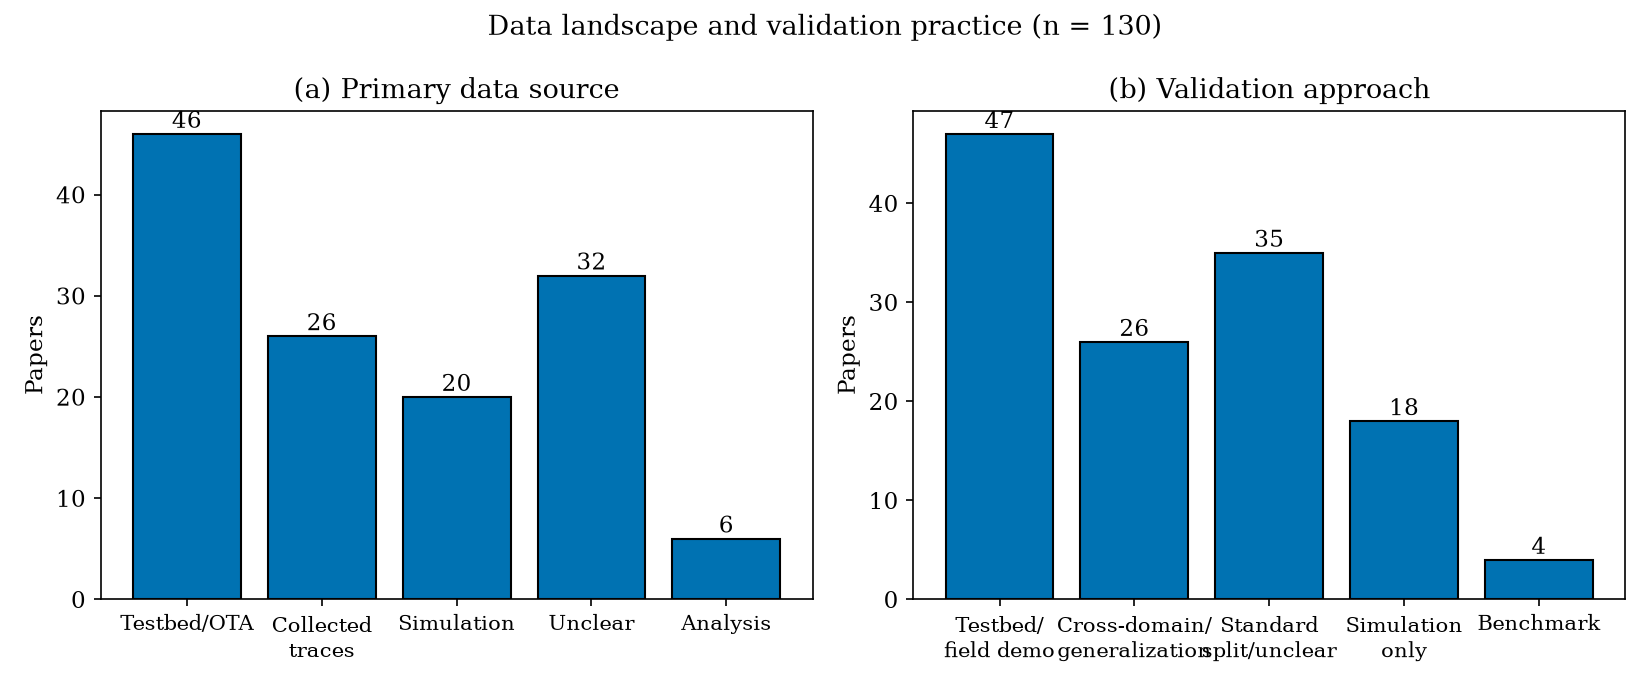
\includegraphics[width=14.0cm]{figures/Fig6_data_validation.png}
\caption{Primary data sources (left) and validation approaches (right) across the corpus (n=130). Testbed/field demonstration is the modal validation; simulation-only work concentrates in key generation (7/12) with a smaller FL-privacy-analysis cluster.}
\label{fig:data}
\end{figure*}


\begin{figure*}[tbp]
\centering
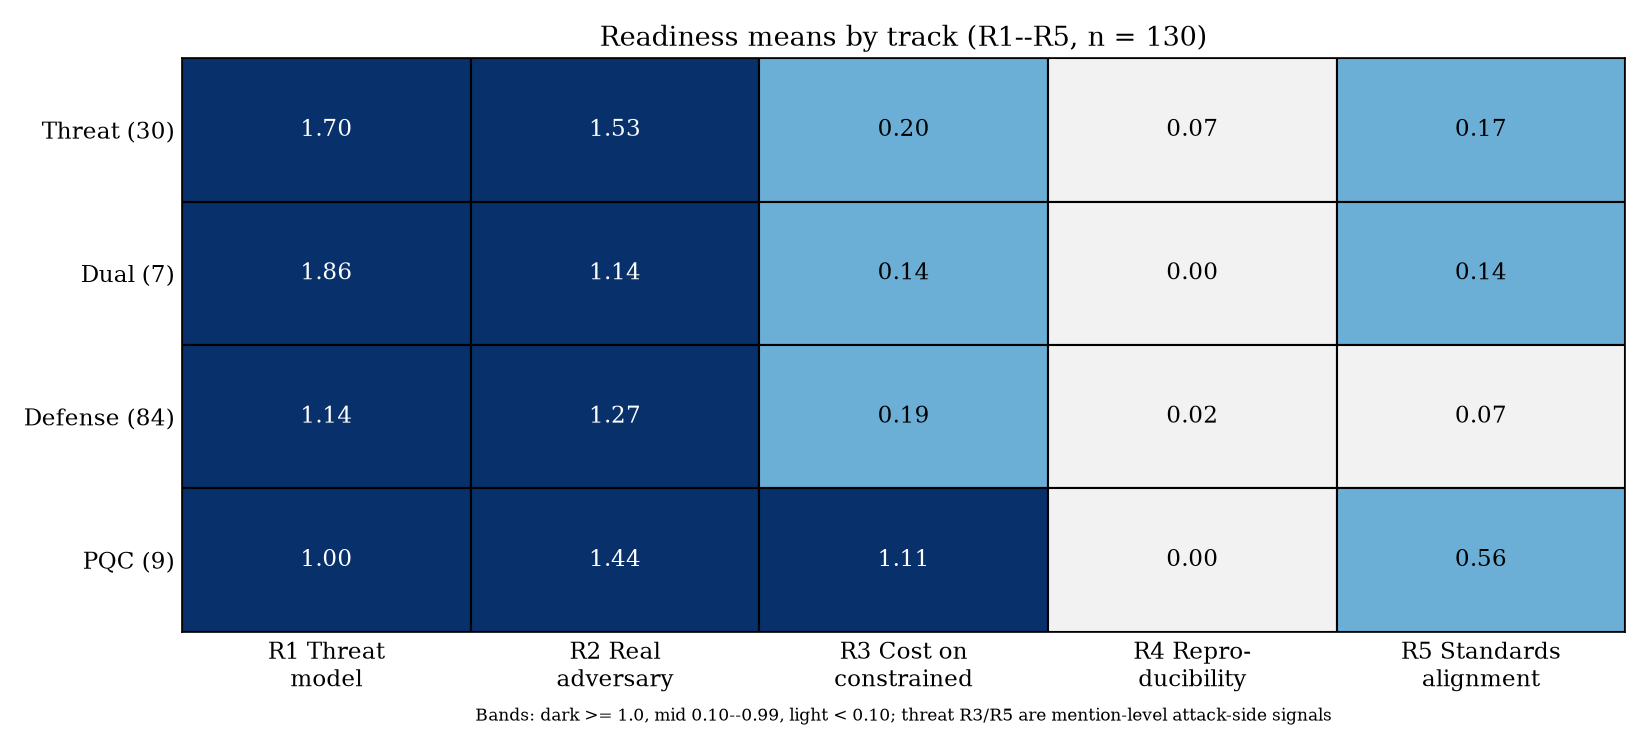
\includegraphics[width=14.0cm]{figures/Fig8_readiness.png}
\caption{Readiness means by track (R1–R5, n=130; bands: dark $\ge$ 1.0, mid 0.10–0.99, light $<$ 0.10; attack-only rows carry R3/R5 only where an observed attacker-cost or standards signal exists—threat R3 0.20, R5 0.17, mention-level; Dual row n=7). Threat work scores realism but releases almost nothing; its standards naming is mention-level. Only the PQC-context stratum reports real onboard costs.}
\label{fig:readiness}
\end{figure*}

Reading these panels together yields the section's headline: the field's empirical base is bifurcated, not uniformly weak. Attacks are demonstrated; defenses are benchmarked. The year-by-year cut shows the evidence grade improving by share: testbed plus cross-domain work rises from about 40\% in 2021–22 to about 60\% in 2023–26 while simulation-only falls from about a quarter to under 10\%—though year arms hold only 10–35 papers each, so these shares are noisy, and absolute simulation-only counts hold roughly flat rather than being displaced.

\subsubsection{Sensitivity analysis: is peer review too slow for AI security?}
\label{sec:sensitivity}
Because the corpus mixes slow and fast publication channels—65 journal papers, 46 conference/workshop papers, and 19 preprints (venue channel coded from confirmed venue strings; \S\ref{sec:methods})—headline findings could in principle be a channel artifact. We therefore ask the question directly: do frontier methods appear first in fast channels, and does journal peer review compensate with stronger validation? The timing answer, within this verified sample, is partial; the rigor answer favors fast channels, noisily.

Frontier methods debut in fast channels, with stated exceptions. Conferences publish the first adversarial-ML paper in 2020 (\upcite{T39} WiseML) a year before the first journal one (2021); the first DRL paper in April 2022 (\upcite{D34} WCNC) a year before the first journal one (April 2023 \upcite{D22}, earliest of the two 2023 journal DRL papers); deep-supervised work debuts tied in 2020 in both channels (\upcite{T01} ASHES workshop and the journal paper \upcite{D81})—\upcite{T01} is the first deep-supervised side-channel threat demonstration in-corpus, not the first fingerprinting paper. Journals lag conferences on adversarial-ML and DRL first appearance only (2 of 4 families); the PQC-context exception is noted (TCHES 2021 \upcite{P05} precedes the in-corpus ACNS 2022 PQC-wireless paper). Table~\ref{tab:firstappear} gives each cell with month granularity. The composition gap persists in shares: adversarial ML is 28\% of conference papers and 37\% of preprints but 31\% of journal papers .

Journals lead conferences on both validation share (testbed 40\% vs 30\%) and mean evaluation-realism scores (R2 1.40 vs 1.26; preprints 1.32, Table~\ref{tab:sensitivity})—but both gaps are small relative to arm sizes (n=65/46/19), and the R2 gap is sensitive to coding judgment (a reconciliation pass moved the means by up to about 0.6), so no prestige gradient is claimed in either direction; the durable channel result is the timing lag, not a rigor ranking. Conferences lead journals by roughly a year on adversarial ML and DRL first appearance (deep-supervised debuts tied in 2020; PQC is reversed with a 2021 journal first). An earliest-public-date audit over all 15 DOI-year mismatches (Crossref online/print dates) moves no first-appearance cell—the \upcite{D22} TVT paper printed April 2023 despite its 2022 DOI number, and \upcite{D36}'s own arXiv dates to April 2021—so the lags stand under both issue-year and earliest-date coding; only \upcite{P05} shifts (December-2020 online-first vs 2021 issue), which widens the PQC reversal. The preprint stratum (37\% testbed, heavily selected—see caveats) cannot carry a channel claim on its own. Consistent with the no-formal-tests rule (\S\ref{sec:methods}), no significance tests are run on these splits.

\begin{table*}[tbp]
\centering
\footnotesize
\caption{First-appearance papers by method family and channel, with issue, online-first, and arXiv-v1 months where evidenced. Lags stand under both issue-year and earliest-date coding except \upcite{P05} (Dec-2020 online-first vs 2021 issue).}
\label{tab:firstappear}
\begin{tabular}{@{}l l p{4.6cm} l@{}}
\toprule
Family & Conference cell & Journal cell & Preprint cell \\
\midrule
Adversarial ML & \upcite{T39} WiseML, Jul 2020 & \upcite{T09} TCCN, Mar 2021 (\upcite{D36} Mar 2022; arXiv Apr 2021) & \upcite{T47} arXiv Jan 2022 \\
Reinforcement/DRL & \upcite{D34} WCNC, Apr 2022 & \upcite{D22} TVT, Apr 2023 (no online-first record) & — \\
Deep supervised & \upcite{T01} ASHES, Nov 2020 & \upcite{D81} IEEE Access 2020 & \upcite{D63} arXiv Jun 2023 \\
PQC implementation & \upcite{P10} LNNS 2025 & \upcite{P05} TCHES 2021 issue (online Dec 2020) & — \\
\bottomrule
\end{tabular}
\end{table*}

\begin{table*}[tbp]
\footnotesize
\centering
\caption{Venue-channel sensitivity: validation mix across journals (n=65), conferences (n=46), and preprints (n=19). Machine-generated from the released dataset.}
\label{tab:sensitivity}
\begin{tabular}{llll}
\toprule
Validation & Journal & Conference & Preprint \\
\midrule
Testbed/field demonstration & 26 (40\%) & 14 (30\%) & 7 (37\%) \\
Cross-domain/generalization & 13 (20\%) & 11 (24\%) & 2 (11\%) \\
Simulation-only & 6 (9\%) & 8 (17\%) & 4 (21\%) \\
Standard split/unclear & 20 (31\%) & 10 (22\%) & 5 (26\%) \\
Benchmark/analysis & 0 & 3 (7\%) & 1 (5\%) \\
\bottomrule
\end{tabular}
\end{table*}


Three caveats bound this finding, and the third is the most serious. First, the preprint arm is small (n=19), the conference arm mixes full conferences with workshops, and each first-appearance cell rests on a single paper in a curated sample at year granularity, so both the shares and the lags carry wide uncertainty. Second, the LLM-assisted family has a single published paper (USENIX Security 2026 \upcite{T28}) and cannot support any channel claim. Third, seeded expert search favors notable, well-evidenced preprints—weak preprints are never found or shortlisted—so the preprint stratum's scores partly reflect selection, not the channel. What selection cannot explain is the journal side of the ledger: journals trail conferences by roughly a year on adversarial ML and DRL first appearance while running close on validation (testbed 40\% vs 30\%; R2 1.40 vs 1.26). For a field where the adversary reads arXiv, that lag is a deployment-relevant result in itself—and it strengthens, rather than weakens, the case for the reporting checklist in \S\ref{sec:gaps}, since speed without standards is how the validation gap in \S\ref{sec:corpus} reproduces itself.

\subsection{AI-enabled threats}
\label{sec:threat}
RFF/authentication attacks form the densest cluster (Table~\ref{tab:representative}): white-box FGSM/PGD and black-box UAP at 81.7\% with $\sim$no victim knowledge on real LoRa captures \upcite{T03}, RL impersonation at $>$90\% from binary feedback \upcite{T18}, GAN-spoofing at 76\% PHY-auth pass \upcite{T09}, backdoors surviving Neural Cleanse/STRIP \upcite{T12} and working model-agnostically \upcite{T16}, self-supervised-target backdoors \upcite{T41}, over-the-air Wi-Fi attacks \upcite{T42}, and fingerprint erasure as privacy attack \upcite{T06}. EM/RF side-channels move key recovery over the air at meters: BLE AES-128 at 15~m from $<$400 traces \upcite{T01}, nRF AES-CCM at 1~m \upcite{T08}, BLE re-keying LTK leakage in $\sim$30 traces. Protocol/traffic attacks show the stack above PHY is equally exposed: padding/shaping defeated by packet-size distributions \upcite{T19}, and LLM-assisted semantic baseband fuzzing (ConSeT: 7 vulns including 3 CVEs across 542 phone models, plus 29 OAI-UE crash sites, USENIX Security 2026 \upcite{T28}).

Critical assessment: attacks are evaluated against real systems with stated—often weak but honest—threat models (strong R2, narrow R1). The missing attack science is adaptive-defense evaluation: most stop at undefended classifiers, which is why Magmaw \upcite{T30} matters—it survives adversarial training, subtraction, detection, and oracle defenses. Domain shift is attack surface, not demonstrated exploit: no cited threat paper exploits shift as a standalone vector.

\begin{table*}[tbp]
\centering
\footnotesize
\setlength{\tabcolsep}{3pt}
\caption{Representative corpus studies by function and method family. Entries gloss each study as: study summary (data basis; headline contribution).}
\label{tab:representative}
\begin{tabular}{@{}>{\raggedright\arraybackslash}p{2.4cm} >{\raggedright\arraybackslash}p{2.4cm} >{\raggedright\arraybackslash}p{9.2cm}@{}}
\toprule
Function & Family & Representative studies \\
\midrule
RFF/auth attack & Adversarial & White-box FGSM/PGD plus black-box UAP 81.7\% on LoRa captures (CNN/LSTM/GRU; no victim knowledge) \upcite{T03}; RL impersonation $>$90\% (SDR; binary feedback) \upcite{T18}; GAN-spoof 76\% (OTA; PHY-auth pass) \upcite{T09}; SSL-target backdoor \upcite{T41}; FooLoc OTA WiFi geofence-bypass \upcite{T42} \\
Side-channel & Deep supervised & Far-field BLE AES-128 at 15~m, $<$400 traces (OTA) \upcite{T01}; nRF AES-CCM at 1~m (RF-SCA) \upcite{T08}; BLE LTK in $\sim$30 traces \\
Protocol/traffic & Fuzzing/ML & LLM baseband fuzzing, 3 CVEs (phones; ConSeT) \upcite{T28}; padding defeat (traces; traffic-shape exploit) \upcite{T19} \\
Universal PHY & Adversarial & Magmaw, NDSS'25 (SDR; protocol-agnostic UAP vs encrypted link) \upcite{T30} \\
Defense RFFI & Robust/open-set & Contrastive, receiver-agnostic, open-set/few-shot, cross-receiver calibration \upcite{D75}, multi-distance \upcite{D73}, satellite PLA \upcite{D71} (captures; accuracy under shift) \\
Keygen & Deep/DRL & KDR/KGR improvements (mostly simulation; reciprocity $+$ IRS/relay) \\
Anti-jamming & DRL $+$ testbed UAV & Relay/power/secrecy-rate control (mixed: 8 testbed, 4 sim-only; costs mostly unreported) \\
PQC-context & Implementation & ML-KEM DTLS 313~ms on ESP32 (hardware; compute fine, bandwidth blocks); WKyber/LAKE (bandwidth attacks) \upcite{P08}\upcite{P11} \\
AI$\times$PQC join & — & Empty in-corpus (non-radio proximity study excluded; recorded gap) \\
\bottomrule
\end{tabular}
\end{table*}

\subsection{AI-assisted defenses}
\label{sec:defense}
RFF/PLA defenses chase domain shift: contrastive embeddings, receiver-agnostic training, open-set/few-shot enrollment, cross-receiver calibration \upcite{D75}, multi-distance generalization \upcite{D73}, domain-adaptive features \upcite{D72}, satellite fingerprinting \upcite{D71}, proactive authentication—accuracy under shift, rarely under attack. Key generation defenses improve KDR/KGR mostly in simulation, with a 2026 channel-informed neural scheme \upcite{D74} grounding features in over-the-air channel soundings. DRL anti-jamming optimizes relay/power/secrecy-rate without onboard-cost reporting. Federated privacy proves differentially private OTA aggregation at small scale.

Critical assessment: the wall between \S\ref{sec:threat} and this section is the finding—dual-track studies are 7 of 130 (5.4\%; 7 of 121 core, 5.8\%), and dual-track realism runs lowest (mean R2 1.14 vs 1.53 threat, 1.27 defense—a 0.13 margin at n=7, so a descriptive remark, not a ranking claim), so closed-loop evaluation exists but is least realistic. RFF accuracy $\ne$ authentication; domain-shift misclassification is attack surface (\upcite{T40}), not demonstrated exploit. The defense literature's strongest protocols (cross-receiver, cross-day, open-set) are exactly the threat literature's attack surface.

\subsection{Quantum-era context}
\label{sec:pqc}
Compute is feasible on ESP32/Pi-class hardware (ML-KEM DTLS 313~ms, beating classical baselines; sub-12~kB Dilithium; Cortex-M4 cycle counts); bandwidth expansion is the blocker; WKyber \upcite{P08} and LAKE \upcite{P11} attack exactly that. Short-range radio key-recovery evidence (far-field BLE SCA \upcite{T01}) shows keys can be pulled over the air, but no in-corpus paper addresses store-now-decrypt-later against the PQC transition for wireless fleets. The AI-threat $\times$ PQC join is empty: no in-corpus paper mounts ML-driven cryptanalysis of a PQC implementation over a radio link (an acoustic–vibration proximity study was excluded for failing the radio-link population; see \S\ref{sec:methods}). The join is recorded as an explicit gap (\S\ref{sec:gaps}), and the stratum stays separate as thesis hygiene requires.

\section{Discussion}
\subsection{Cross-cutting directions}
\label{sec:cross}
Closed-loop evaluation—defined here as dual-track studies plus any threat paper that
evaluates against a stated defense and any defense paper that evaluates against a stated
attack—reaches at least 14 of 121 core studies (11.6\%). This is a lower bound: abstract
wording may hide further cases, a full-text audit is future work, and the construct is
hand-judged with no separate reliability estimate. The figure decomposes into 7 dual-track
papers \upcite{D08,D36,D37,T05,T11,T14,T46} (5 under a stricter title-only rule), 3 threat papers that demonstrate against defenses
(including one that survives adversarial training, subtraction, detection and oracle defenses,
one that bypasses two published detection methods, and one that assesses a distillation defense
on an over-the-air testbed), and 4 defense papers that demonstrate against attacks (GAN-based
impersonation, Byzantine poisoning, live impersonating unmanned aerial vehicles, and evasive
queries). The broader measure remains the exception (the \S\ref{sec:threat}–\S\ref{sec:defense} wall), autonomous trust (real-time deadlines unbenchmarked; OTA crypto-agility essentially unaddressed; multi-agent trust in 1–2 papers while FL-for-drones falls to deauth$\rightarrow$impersonation chaining \upcite{T36}), and reproducibility (4 verified artifact releases among 121 core, 3.3\%) are the three cross-cutting threads (Fig.~\ref{fig:gaps}). Dual-track realism is lowest (mean R2 1.14, n=7—a 0.13 margin over defense, fragile at this n), which complicates any closed-loop optimism: evaluation exists but is least realistic. Function $\times$ validation cross-tabulations are descriptive (no significance tests; metric heterogeneity forbids pooling). The field optimizes estimators while adversaries optimize exploitability—a mismatch no single-function advance can fix.

A venue-community check does not explain the asymmetry away: stratifying R2 by security venues (NDSS, CCS, USENIX, TIFS, WiseML and kin) versus comms and other venues, comms-venue threats outscore comms-venue defenses on realism (means 1.61 vs 1.31, n=23/68), while security-venue papers score lower in both tracks (threat 1.29, n=7—\upcite{T01,T19,T20,T23,T28,T30,T39}, of which \upcite{T01,T28} and \upcite{T30} score 2 and the analysis/workshop remainder scores 0–1; defense 1.12, n=16)—small-n and caution-worthy, but running against the community-norms confound rather than with it. Fig.~\ref{fig:layered} stacks the corpus by layer to make the coverage gap visible: the signal layer is contested, the link layer half-defended, the protocol layer thinly covered, and the system layer essentially absent.
\begin{figure*}[tbp]
\centering
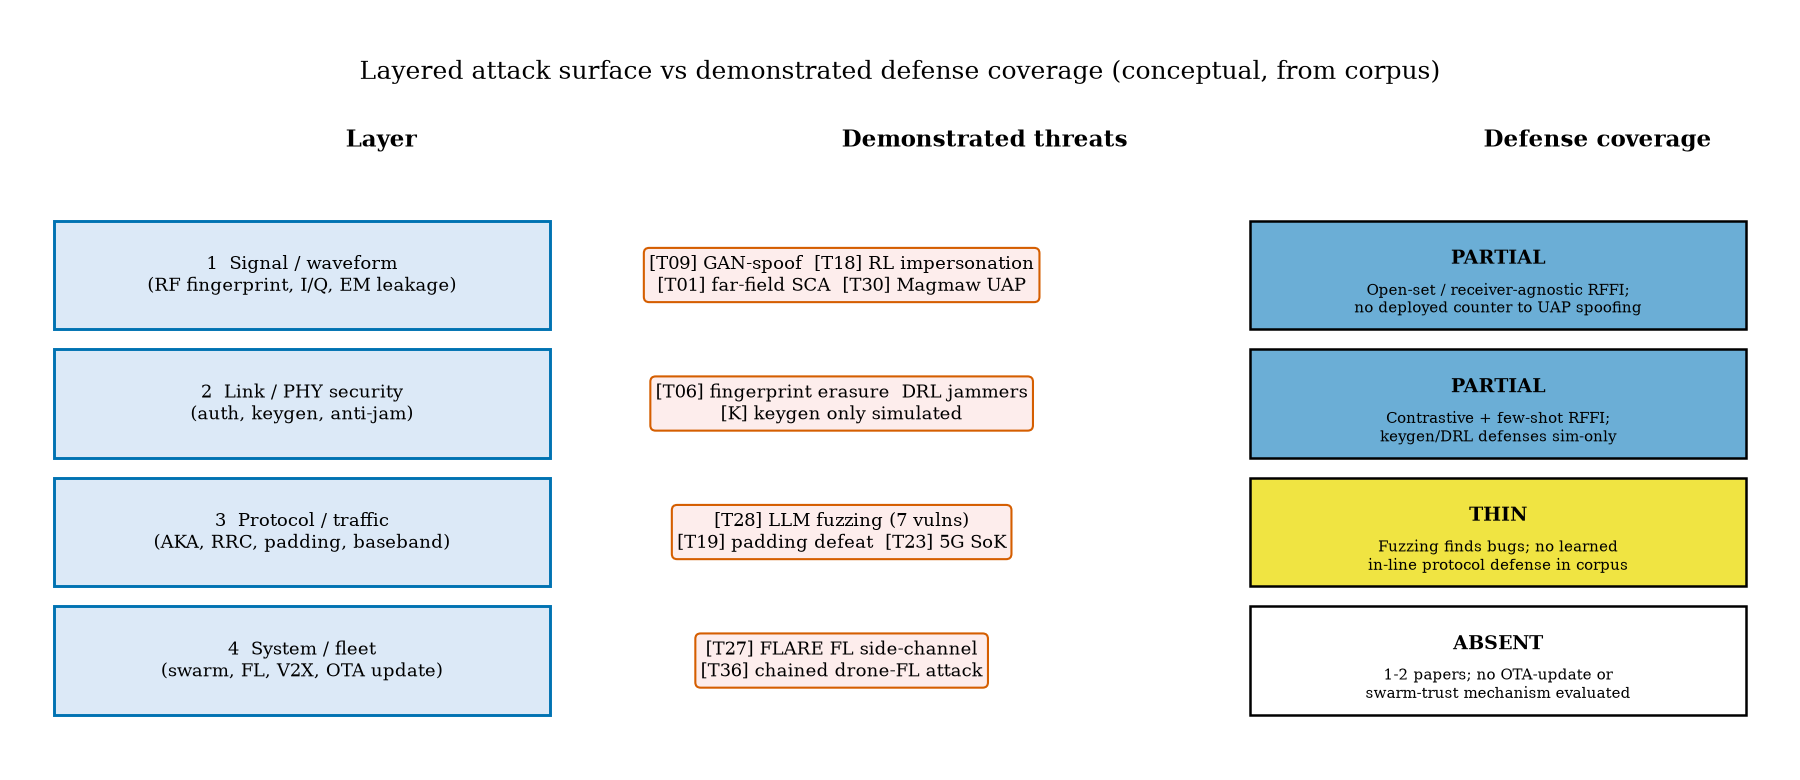
\includegraphics[width=15.2cm]{figures/FigD_layered_coverage.png}
\caption{Layered attack surface versus demonstrated defense coverage, synthesized from the corpus (conceptual). Coverage thins with every step up the stack.}
\label{fig:layered}
\end{figure*}

\begin{figure*}[tbp]
\centering
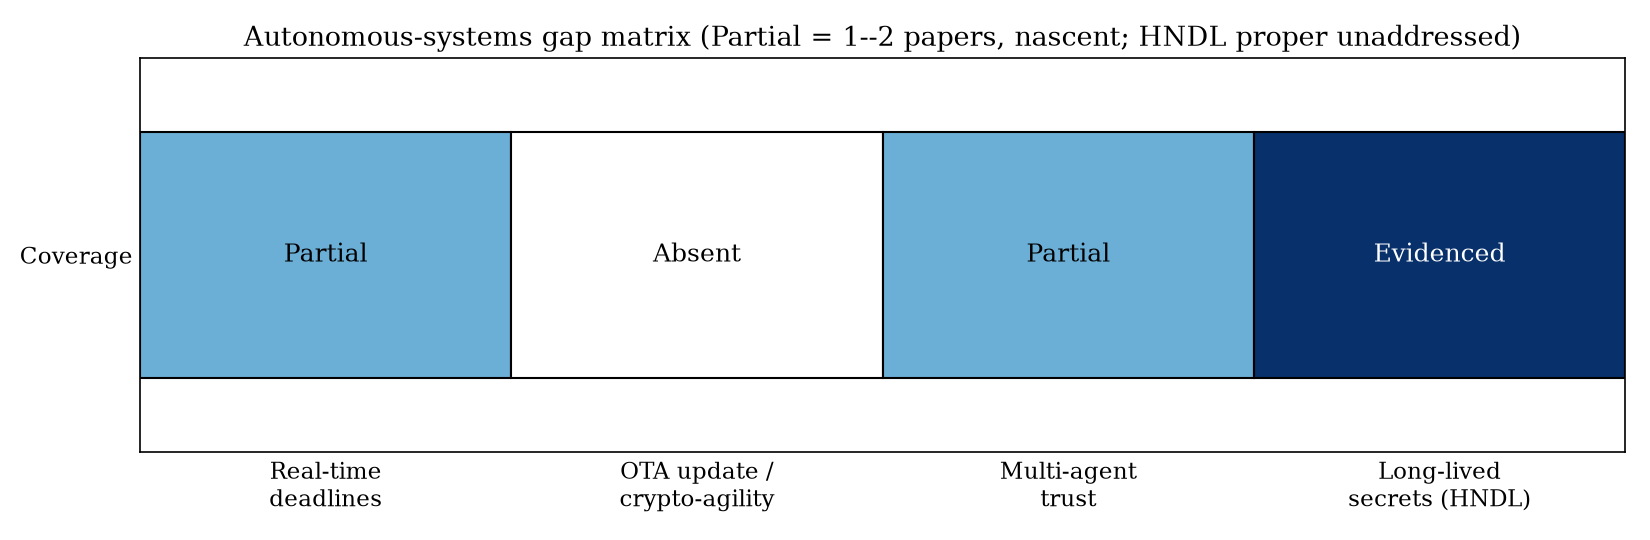
\includegraphics[width=14.0cm]{figures/Fig9_gap_matrix.png}
\caption{Autonomous-systems gap matrix. Real-time deadlines and multi-agent trust are Partial (1–2 papers each: nascent coverage, far from deployment-grade, hence “essentially unaddressed” in the abstract); OTA update/crypto-agility is absent; long-lived secrets show short-range key-recovery evidence (BLE far-field SCA) while store-now-decrypt-later against the PQC transition is unaddressed.}
\label{fig:gaps}
\end{figure*}

\subsection{Research gaps and future directions}
\label{sec:gaps}
Cross-referencing the bibliometric analysis of \S\ref{sec:corpus} with the function-level reviews of \S\S\ref{sec:threat}–\ref{sec:cross} yields six structural gaps, summarized in Table~\ref{tab:gaps} and operationalized into the concrete reporting checklist in Table~\ref{tab:checklist}. The ordering is deliberate: the first three rows concern how the field evaluates and shares evidence, the fourth how it reports cost, and the last two where the evidence stops short of deployment needs. None of the six requires a new method family, and all are measurable against the released dataset—a rerun of this review in two years should be able to score each row as narrowed, unchanged, or widened. The checklist is the review's most actionable artifact: the minimum metadata a study must disclose for its claims to be comparable, reproducible, and poolable in future syntheses. Each item corresponds to a practice whose absence the corpus analysis showed to be distorting—undisclosed splits, unnamed datasets, or unquantified compute. Checklist adherence in-corpus is reported only for coded items (descriptive): dataset/testbed identity present for 72 testbed-or-collected rows with 32 unclear; adversary model explicit (R1=2) in 39 of 130; split protocol rarely isolated (35 standard/unclear validations); OTA-vs-simulation declared via validation field (47 testbed, 18 sim-only); closed-loop (item 6) at 14 of 121 core (11.6\%) by the rule in \S\ref{sec:cross}; onboard cost present on 16 of 84 defense rows (defense R3 mean 0.19); artifacts released for 4 of 121 core (3.3\%). Items 7–9 and 11 (baselines, seeds, uncertainty, failure analysis) were never coded, so no corpus claim is made about them—they are prospective requirements, as is the checklist as a whole beyond the coded items.
\begin{table*}[tbp]
\centering
\footnotesize
\setlength{\tabcolsep}{3pt}
\caption{Structural research gaps and corresponding future directions.}
\label{tab:gaps}
\begin{tabular}{@{}>{\raggedright\arraybackslash}p{3.0cm} >{\raggedright\arraybackslash}p{5.2cm} >{\raggedright\arraybackslash}p{6.4cm}@{}}
\toprule
Gap & Evidence & Direction \\
\midrule
Closed-loop evaluation & Dual-track 7/130 (5.4\%); dual R2 1.14 lowest (margin 0.13 at n=7); broader measure 14/130 & Adversarial-benchmark suites with OTA mandates \\
Reproducibility & 3.3\% verified releases (4/121 core); R4 means 0.00–0.07 & Artifact-evaluated security tracks; dataset DOIs \\
Standards alignment & 9.9\% outside PQC (13.1\% incl. PQC); RFF 6/69; defense R5 0.07 & Authentication profiles (3GPP/IETF) for learned PHY-auth \\
Onboard cost & DRL/semantic cost-silent; defense R3 0.19 (16/84 rows) & Latency/energy/memory as required reporting \\
Autonomous trust & 1–2 papers per need & Real-time auth, OTA agility, swarm insider models \\
AI$\times$PQC join & Empty in-corpus (non-radio proximity study excluded) & ML-SCA of PQC over the air; migration prioritization \\
\bottomrule
\end{tabular}
\end{table*}

\begin{table*}[tbp]
\centering
\footnotesize
\setlength{\tabcolsep}{3pt}
\caption{Proposed WIRELESS-AI-RC reporting checklist (12 items).}
\label{tab:checklist}
\begin{tabular}{@{}l >{\raggedright\arraybackslash}p{3.8cm} >{\raggedright\arraybackslash}p{10.0cm}@{}}
\toprule
\# & Item & Must report \\
\midrule
1 & Dataset/testbed identity & Name, version, download or testbed description \\
2 & Device/link population & Radios, channels, distances, day/receiver splits \\
3 & Adversary model & Knowledge, capability, RF/compute budget \\
4 & Split protocol & Within/cross-receiver/day/domain $+$ isolation argument \\
5 & OTA vs simulation & Declaration; sim-only flagged as such \\
6 & Closed-loop evaluation & Attack paper: defenses tested; defense paper: attacks tested \\
7 & Baselines & $\ge$1 classical alongside proposed method, identical data \\
8 & Randomness & Seeds or repeated-run statistics \\
9 & Uncertainty & Error bars, not point estimates alone \\
10 & Onboard cost & Latency/energy/memory on stated platform \\
11 & Failure analysis & $\ge$1 documented failure mode $+$ distribution \\
12 & Artifacts & Code/data DOI or explicit exemption \\
\bottomrule
\end{tabular}
\end{table*}
We suggest venues adopt the checklist as a submission requirement and authors attach it to their released datasets: it costs little, and it is what lets the next synthesis do its job.

\section{Conclusion}
\label{sec:conclusion}
Three conclusions stand out, answering the title question for the research literature directly: no—the published literature does not demonstrate wireless security ready for the AI era on current evidence (a statement about literature maturity in this curated sample, not a measurement of deployed systems). First, the method center moved from fingerprint classifiers to adversarial science—attacks are cheap, largely demonstrated on captures/testbeds (threat plurality up to 16 of 30 testbed, not norm), and over-the-air demonstrated in the strongest cases. That contrast is descriptively striking but rests on the least reliable field in the corpus (validation, $\kappa = 0.21$), so it is reported as a bound rather than as a precise count. Second, the application center stayed in RFFI accuracy, which is not authentication—defenses are rarely adversarially evaluated (broader closed-loop 14/121 core (11.6\%); dual-track detail in \S\ref{sec:cross}). Third, readiness does not follow publication volume: reproducibility, standards, onboard cost, and autonomous-trust evidence trail accuracy claims in volume and maturity—and venue channels differ modestly on rigor: validation rigor runs close across channels (testbed 40\% journals vs 30\% conferences; R2 1.40 vs 1.26, gaps small relative to arm sizes) (\S\ref{sec:sensitivity}). If the last five years were about discovering what learning can extract from radio signals, the next five will be decided by what it can be trusted to protect—under adaptive adversaries, on constrained radios, at fleet scale.

\appendix
\section{Included studies}
\begin{table*}[p]
\centering
\scriptsize
\setlength{\tabcolsep}{2.5pt}
\caption{Included studies (part 1 of 2): reference number, corpus ID, first author, year, publication venue, track (D defense, T threat, B dual, Q post-quantum context) and security function.}
\label{tab:corpus}
\begin{tabular}{@{}lllll>{\raggedright\arraybackslash}p{3.3cm}>{\raggedright\arraybackslash}p{1.9cm}@{}}
\toprule
No. & ID & Author & Year & Venue & Tr. & Function \\
\midrule
1 & T03 & Ma & 2026 & IEEE Transactions on Mobile Computing vol 25 pp 7831-7844 & T & RFFI/auth \\
2 & T18 & Karunaratne & 2021 & IEEE ICC 2021 & T & RFFI/auth \\
3 & T09 & Shi & 2021 & IEEE Trans Cogn Commun Netw & T & RFFI/auth \\
4 & T01 & Wang & 2020 & 4th ACM Workshop on Attacks and Solutions in Hardware Security (ASHES@CCS) & T & Side-chan. \\
5 & T30 & Chang & 2025 & NDSS & T & Primitive \\
9 & T05 & Sagduyu & 2023 & IEEE MILCOM 2023 (preliminary); full version 2024 & B & RFFI/auth \\
10 & T14 & Shi & 2023 & IEEE Trans Mobile Computing & B & RFFI/auth \\
11 & D55 & Hanna & 2021 & IEEE Trans Cogn Commun Networking vol 7 pp 59-72 & D & RFFI/auth \\
12 & T15 & al. & 2021 & IEEE GLOBECOM 2021 & T & RFFI/auth \\
13 & D20 & Cheng & 2025 & IEEE Transactions on Vehicular Technology & D & RFFI/auth \\
14 & T20 & Morales & 2023 & ACM CPS-IoT Week (pp 19-24) & T & Protocol \\
15 & T41 & Yao & 2025 & IEEE Trans Inf Forensics Secur & T & RFFI/auth \\
16 & T42 & Xiao & 2023 & venue unconfirmed (arXiv 2301.03760) & T & RFFI/auth \\
17 & T44 & Ke & 2024 & IEEE Trans Inf Forensics Secur & T & Protocol \\
18 & T28 & Huang & 2026 & 35th USENIX Security Symposium 2026 (pp 457-476) & T & Protocol \\
20 & T40 & Cao & 2025 & IEEE MILCOM & T & RFFI/auth \\
21 & T39 & Restuccia & 2020 & ACM WiseML (2nd Workshop Wireless Secur Mach Learn) & T & RFFI/auth \\
22 & D34 & Abdalla & 2022 & IEEE WCNC & D & Anti-jam \\
23 & D22 & Dong & 2023 & IEEE Trans Vehicular Technology (Apr) & D & Anti-jam \\
24 & D81 & Wang & 2020 & IEEE Access & D & RFFI/auth \\
25 & P05 & Greconici & 2021 & IACR TCHES & Q & PQC migration (contextual) \\
26 & D36 & Sahay & 2022 & IEEE Trans Cogn Commun Networking (Mar 2022) & B & Protocol \\
27 & T47 & Shi & 2022 & arXiv & T & Anti-jam \\
28 & D63 & Wang & 2023 & venue unconfirmed (arXiv 2306.13895) & D & RFFI/auth \\
29 & P10 & Blanco-Romero & 2025 & Lecture Notes in Networks and Systems (book chapter) & Q & PQC migration (contextual) \\
30 & T12 & Zhao & 2023 & IEEE ICCCN & T & RFFI/auth \\
31 & T16 & Zhao & 2024 & IEEE INFOCOM Workshops & T & RFFI/auth \\
32 & T06 & Lu & 2025 & IEEE Trans Network Science and Engineering 2025 & T & RFFI/auth \\
33 & T08 & Ji & 2025 & IEEE ISMVL & T & Side-chan. \\
34 & T19 & Engelberg & 2022 & ACM WPES & T & RFFI/auth \\
35 & D75 & He & 2026 & venue unconfirmed (arXiv 2603.08402) & D & RFFI/auth \\
36 & D73 & Ahmed & 2025 & IEEE PIMRC & D & RFFI/auth \\
37 & D71 & Oligeri & 2022 & IEEE Trans Inf Forensics Secur & D & RFFI/auth \\
38 & P08 & Gonzalez de la Torre & 2025 & IEEE Access & Q & PQC migration (contextual) \\
39 & P11 & Nasiraee & 2025 & Int Conf Combinatorics Cryptography Comput Sci (via eprint 2025/2293) & Q & PQC migration (contextual) \\
40 & D72 & Elmaghbub & 2024 & IEEE Trans Mach Learn Commun Netw & D & RFFI/auth \\
41 & D74 & Sanchez Viloria & 2026 & venue unconfirmed (arXiv 2609.16341) & D & Keygen \\
42 & D08 & Papangelo & 2024 & IEEE Communications Magazine vol 62(11) pp 108-113 & B & RFFI/auth \\
43 & D37 & Meng & 2025 & IEEE Trans Inf Forensics Secur vol 20 pp 3731-3744 & B & Protocol \\
44 & T11 & Huang & 2024 & IEEE Trans ML in Commun Networking & B & RFFI/auth \\
45 & T46 & Li & 2026 & J Cyber Secur Mobility & B & Protocol \\
46 & T36 & Sabo & 2026 & venue unconfirmed (arXiv 2607.20280) & T & RFFI/auth \\
47 & T23 & Eleftherakis & 2025 & ACM WiSec & T & Protocol \\
48 & D24 & Seif & 2020 & IEEE ISIT 2020 (pp 2604-2609) & D & FL/privacy \\
49 & D11 & Zhang & 2021 & IEEE Internet of Things Journal & D & Keygen \\
50 & D12 & Jiao & 2021 & ACM WiseML & D & Keygen \\
51 & D25 & Aghdam & 2021 & IEEE CAMAD Workshops & D & FL/privacy \\
52 & D54 & Huang & 2021 & IEEE ICC Workshops & D & FL/privacy \\
53 & D56 & Shen & 2021 & IEEE J Sel Areas Commun vol 39 pp 2604-2616 & D & RFFI/auth \\
54 & D78 & Zhang & 2021 & IEEE Vehicular Technology Conference & D & RFFI/auth \\
55 & D82 & Wei & 2021 & arXiv & D & FL/privacy \\
56 & D83 & Elgabli & 2021 & IEEE Transactions on Communications & D & FL/privacy \\
57 & D85 & Chen & 2021 & arXiv & D & FL/privacy \\
58 & D86 & Seif & 2021 & IEEE International Symposium on Information Theory (ISIT) & D & FL/privacy \\
59 & D88 & Yang & 2021 & IEEE Journal on Selected Areas in Communications & D & FL/privacy \\
60 & T25 & Xie & 2021 & URSI GASS 2021 & T & Primitive \\
61 & D05 & Li & 2022 & IEEE ISCC & D & RFFI/auth \\
62 & D09 & Feng & 2022 & IEEE VTC Spring & D & Keygen \\
63 & D57 & Rajendran & 2022 & IEEE Trans Inf Forensics Secur vol 17 pp 1285-1299 & D & RFFI/auth \\
64 & P03 & Abdulrahman & 2022 & ACNS (LNCS) & Q & PQC migration (contextual) \\
65 & T38 & Bao & 2022 & IEEE Internet of Things Journal vol 9 pp 9012-9024 & T & RFFI/auth \\
66 & D01 & al. & 2023 & Engineering Applications of Artificial Intelligence (Elsevier) & D & Protocol \\
67 & D03 & Wang & 2023 & IEEE NCIC & D & Keygen \\
68 & D06 & Lu & 2023 & IEEE NNICE & D & RFFI/auth \\
69 & D10 & Chen & 2023 & IEEE ICC & D & Keygen \\\bottomrule
\end{tabular}
\end{table*}
\begin{table*}[p]
\centering
\scriptsize
\setlength{\tabcolsep}{2.5pt}
\caption{Included studies (part 2 of 2): reference number, corpus ID, first author, year, publication venue, track (D defense, T threat, B dual, Q post-quantum context) and security function.}
\label{tab:corpusb}
\begin{tabular}{@{}lllll>{\raggedright\arraybackslash}p{3.3cm}>{\raggedright\arraybackslash}p{1.9cm}@{}}
\toprule
No. & ID & Author & Year & Venue & Tr. & Function \\
\midrule
70 & D13 & Shi & 2023 & IEEE NCIC & D & Keygen \\
71 & D15 & Lv & 2023 & IEEE Trans Wireless Commun vol 22(12) & D & Anti-jam \\
72 & D19 & Amin & 2023 & IEEE ISNCC & D & RFFI/auth \\
73 & D23 & Zhang & 2023 & IEEE Trans Dependable Secure Comput & D & FL/privacy \\
74 & D35 & Hoseini & 2023 & IEEE GLOBECOM Workshops & D & Anti-jam \\
75 & D50 & Puppo & 2023 & IEEE ISCC & D & RFFI/auth \\
76 & D58 & Jagannath & 2023 & IEEE Trans Cogn Commun Networking vol 9 pp 940-949 & D & RFFI/auth \\
77 & D79 & Ma & 2023 & IEEE Wireless Communications and Networking Conference & D & RFFI/auth \\
78 & T04 & Liu & 2023 & IEEE Wireless Communications Letters vol 12(6) & T & RFFI/auth \\
79 & T43 & Huang & 2023 & IEEE Ucom & T & RFFI/auth \\
80 & D04 & Dentremont & 2024 & IEEE IWCMC & D & RFFI/auth \\
81 & D07 & Shen & 2024 & IEEE Trans Mobile Computing & D & RFFI/auth \\
82 & D14 & Liu & 2024 & IEEE WCNC & D & Anti-jam \\
83 & D16 & Shao & 2024 & IEEE Trans Mobile Computing vol 23(12) & D & Anti-jam \\
84 & D17 & Su & 2024 & IEEE ICOIN & D & Anti-jam \\
85 & D26 & Mao & 2024 & IEEE ICC (presented per authors) & D & Anti-jam \\
86 & D33 & Tyler & 2024 & venue unconfirmed (arXiv 2411.10287) & D & Primitive \\
87 & D38 & Gao & 2024 & IEEE Wireless Communications & D & Keygen \\
88 & D39 & Alwazani & 2024 & venue unconfirmed (arXiv 2409.15303) & D & Keygen \\
89 & D41 & Zhang & 2024 & IEEE Trans Vehicular Technology (accepted per arXiv) & D & Keygen \\
90 & D44 & Chen & 2024 & IEEE ICC & D & RFFI/auth \\
91 & D47 & Parpart & 2024 & IEEE MILCOM & D & RFFI/auth \\
92 & D53 & Li & 2024 & IEEE Communications Letters & D & Protocol \\
93 & D59 & Jiang & 2024 & IEEE Trans Wireless Commun vol 23 pp 2070-2081 & D & RFFI/auth \\
94 & D62 & Hu & 2024 & IET Communications vol 18 & D & RFFI/auth \\
95 & D64 & Zhao & 2024 & IEEE INFOCOM (pp 2099-2108) & D & RFFI/auth \\
96 & D65 & Zhao & 2024 & ACM MobiCom (pp 2389-2394) & D & RFFI/auth \\
97 & D66 & Yin & 2024 & IEEE Trans Cogn Commun Networking & D & RFFI/auth \\
98 & D70 & Elmaghbub & 2024 & ACM WiSec & D & RFFI/auth \\
99 & D77 & Yin & 2024 & IEEE Trans Green Commun Netw & D & Anti-jam \\
100 & D87 & Tavangaran & 2024 & IET Communications & D & FL/privacy \\
101 & P04 & Kim & 2024 & IEEE Access & Q & PQC migration (contextual) \\
102 & T17 & Zhang & 2024 & IEEE Trans ML in Commun Networking & T & RFFI/auth \\
103 & T31 & al. & 2024 & ACM WiSec & T & Anti-jam \\
104 & D02 & Guo & 2025 & IEEE Trans Inf Forensics Secur & D & RFFI/auth \\
105 & D18 & Zhou & 2025 & IEEE Trans Wireless Commun vol 24 pp 2722-2733 & D & RFFI/auth \\
106 & D21 & Song & 2025 & IEEE Trans Consumer Electronics (Nov) & D & Anti-jam \\
107 & D27 & Wu & 2025 & IEEE Wireless Commun Lett (Mar) & D & RFFI/auth \\
108 & D28 & Xie & 2025 & IEEE Internet of Things Journal vol 12 pp 25691-25706 & D & RFFI/auth \\
109 & D29 & Liu & 2025 & IEEE Commun Lett (Sep) & D & RFFI/auth \\
110 & D30 & Cai & 2025 & IEEE ICC & D & RFFI/auth \\
111 & D31 & Ma & 2025 & Sensors & D & RFFI/auth \\
112 & D32 & Huang & 2025 & IEEE Internet of Things Journal & D & RFFI/auth \\
113 & D40 & Guo & 2025 & IEEE WCSP & D & Keygen \\
114 & D42 & Shahiri & 2025 & venue unconfirmed (arXiv 2507.00714; under review) & D & Keygen \\
115 & D43 & Chen & 2025 & IEEE ICNC 2025 (pp 436-440) & D & Anti-jam \\
116 & D48 & Mahajan & 2025 & IEEE ICASSP (per arXiv comment) & D & RFFI/auth \\
117 & D49 & Johnson & 2025 & IEEE Network & D & RFFI/auth \\
118 & D52 & Amiriara & 2025 & IEEE Trans Cogn Commun Networking vol 11 pp 2955-2969 & D & Anti-jam \\
119 & D60 & Kong & 2025 & IEEE Trans Inf Forensics Secur & D & RFFI/auth \\
120 & D61 & Yang & 2025 & IEEE Trans Mobile Computing (Nov) & D & RFFI/auth \\
121 & D67 & Pei & 2025 & IEEE TrustCom (pp 556-565) & D & RFFI/auth \\
122 & D68 & Li & 2025 & IEEE ISCC & D & RFFI/auth \\
123 & D80 & Jawne & 2025 & FutureG Symposium & D & RFFI/auth \\
124 & P01 & Lopez & 2025 & IEEE QCE & Q & PQC migration (contextual) \\
125 & P06 & Nguyen & 2025 & IEEE Trans Circuits and Systems I (Feb) & Q & PQC migration (contextual) \\
126 & T21 & Nakhla & 2025 & IEEE World AI IoT Congress (May) & T & Protocol \\
127 & T22 & Haydar & 2025 & IEEE NTMS 2025 (Paris) & T & RFFI/auth \\
128 & D45 & Razak & 2026 & venue unconfirmed (arXiv 2605.15593) & D & RFFI/auth \\
129 & D46 & Zeng & 2026 & venue unconfirmed (arXiv 2608.04881; INFOCOM-2026 submission label inconsistent with Aug-2026 posting) & D & RFFI/auth \\
130 & D69 & Yang & 2026 & IEEE Trans Mobile Computing (Feb) & D & RFFI/auth \\
131 & D76 & Liu & 2026 & venue unconfirmed (arXiv 2604.24022) & D & RFFI/auth \\
132 & D84 & Ayli & 2026 & arXiv & D & FL/privacy \\
133 & P09 & Kudaloor & 2026 & IEEE Communications Standards Magazine (accepted) & Q & PQC migration (contextual) \\
134 & T27 & Shuvo & 2026 & IEEE INFOCOM & T & RFFI/auth \\\bottomrule
\end{tabular}
\end{table*}

\begin{acknowledgement}
The authors thank the maintainers of the Crossref, arXiv and OpenAlex APIs, on whose records the
retrieval described in \S\ref{sec:methods} depends.
\end{acknowledgement}


\begin{thebibliography}{999}
\small
\bibitem[1]{T03}
J. Ma, J. Zhang, G. Shen, A. Marshall, and C.-H. Chang, Adversarial Attacks Against Deep Learning-Based Radio Frequency Fingerprint Identification, \emph{IEEE Transactions on Mobile Computing}, vol. 25, pp. 7831–7844, 2026, doi: 10.1109/TMC.2025.3646257.
\bibitem[2]{T18}
S. Karunaratne, E. Krijestorac, and D. Cabric, Penetrating RF Fingerprinting-based Authentication with a Generative Adversarial Attack, \emph{IEEE ICC 2021}, 2021, doi: 10.1109/ICC42927.2021.9500893.
\bibitem[3]{T09}
Y. Shi, K. Davaslioglu, and Y. E. Sagduyu, Generative Adversarial Network in the Air: Deep Adversarial Learning for Wireless Signal Spoofing, \emph{IEEE Trans Cogn Commun Netw}, 2021, doi: 10.1109/tccn.2020.3010330.
\bibitem[4]{T01}
R. Wang, H. Wang, and E. Dubrova, Far Field EM Side-Channel Attack on AES Using Deep Learning, \emph{4th ACM Workshop on Attacks and Solutions in Hardware Security (ASHES@CCS)}, 2020, doi: 10.1145/3411504.3421214.
\bibitem[5]{T30}
J.-W. Chang, K. Sun, et al., Magmaw: Modality-Agnostic Adversarial Attacks on Machine Learning-Based Wireless Communication Systems, \emph{NDSS}, 2025, doi: 10.14722/ndss.2025.23336.
\bibitem[6]{B03}
A. Jagannath, J. Jagannath, et al., A Comprehensive Survey on Radio Frequency (RF) Fingerprinting: Traditional Approaches, Deep Learning, and Open Challenges, \emph{Computer Networks (Elsevier)}, 2022, \url{https://arxiv.org/abs/2201.00680}.
\bibitem[7]{B07}
et al., Adversarial Machine Learning in Wireless Communications Using RF Data: A Review, \emph{IEEE Communications Surveys \& Tutorials}, 2022, doi: 10.1109/COMST.2022.3205184.
\bibitem[8]{B02}
T. M. Hoang, A. Vahid, H. D. Tuan, and L. Hanzo, Physical Layer Authentication and Security Design in the Machine Learning Era, \emph{IEEE Communications Surveys \& Tutorials}, vol. 26, no. 3, 2024, \url{https://ieeexplore.ieee.org/document/10428002}.
\bibitem[9]{T05}
Y. E. Sagduyu and T. Erpek, Adversarial Attack and Defense for LoRa Device Identification and Authentication via Deep Learning, \emph{IEEE MILCOM 2023 (preliminary); full version 2024}, 2023, \url{https://arxiv.org/abs/2412.21164}.
\bibitem[10]{T14}
Y. Shi and Y. E. Sagduyu, Membership Inference Attack and Defense for Wireless Signal Classifiers with Deep Learning, \emph{IEEE Trans Mobile Computing}, 2023, doi: 10.1109/tmc.2022.3148690.
\bibitem[11]{D55}
S. Hanna, S. Karunaratne, and D. Cabric, Open Set Wireless Transmitter Authorization: Deep Learning Approaches and Dataset Considerations, \emph{IEEE Trans Cogn Commun Networking}, vol. 7, pp. 59–72, 2021, doi: 10.1109/tccn.2020.3043332.
\bibitem[12]{T15}
et al., Open Set RF Fingerprinting using Generative Outlier Augmentation, \emph{IEEE GLOBECOM 2021}, 2021, \url{https://arxiv.org/abs/2108.13099}.
\bibitem[13]{D20}
Q. Cheng, et al., Physical Layer Authentication in UAV Communications (spoofing), \emph{IEEE Transactions on Vehicular Technology}, 2025, doi: 10.1109/tvt.2025.3532982.
\bibitem[14]{T20}
Morales, Bienek-Parrish, Jenkins, and Slavin, Protocol-agnostic IoT Device Classification on Encrypted Traffic, \emph{ACM CPS-IoT Week ()}, pp. 19–24, 2023, doi: 10.1145/3576914.3587487.
\bibitem[15]{T41}
Z. Yao and G. Gui, Backdoor Attack on Self-Supervised Learning-Based RFF Identification Using Spectrum Enhanced Insensitive Perturbation Trigger, \emph{IEEE Trans Inf Forensics Secur}, 2025, doi: 10.1109/tifs.2025.3577013.
\bibitem[16]{T42}
F. Xiao, Y. Huang, Y. Zuo, and W. Kuang, Over-The-Air Adversarial Attacks on Deep Learning Wi-Fi Fingerprinting (FooLoc), \emph{venue unconfirmed (arXiv 2301.03760)}, 2023, \url{https://arxiv.org/abs/2301.03760}.
\bibitem[17]{T44}
D. Ke, X. Wang, and Z. Huang, Frequency-Selective Adversarial Attack Against Deep Learning-Based Wireless Signal Classifiers, \emph{IEEE Trans Inf Forensics Secur}, 2024, doi: 10.1109/tifs.2024.3352423.
\bibitem[18]{T28}
Q. Huang, X. Wang, W. Guo, G. Gu, and H. Hu, Semantics Over Syntax: Uncovering Pre-Authentication 5G Baseband Vulnerabilities, \emph{35th USENIX Security Symposium 2026 ()}, pp. 457–476, 2026, \url{https://www.usenix.org/conference/usenixsecurity26/presentation/huang-qiqing}.
\bibitem[19]{T07}
et al., RANsacked: A Domain-Informed Approach for Fuzzing LTE and 5G RAN-Core Interfaces, \emph{ACM CCS 2024}, 2024, doi: 10.1145/3658644.3670320.
\bibitem[20]{T40}
X. Cao, B. Adhikari, S. Zhao, and J. Wu, An Adversarial-Driven Experimental Study on Deep Learning for RF Fingerprinting, \emph{IEEE MILCOM}, 2025, doi: 10.1109/milcom64451.2025.11309917.
\bibitem[21]{T39}
F. Restuccia, et al., Generalized wireless adversarial deep learning, \emph{ACM WiseML (2nd Workshop Wireless Secur Mach Learn)}, 2020, doi: 10.1145/3395352.3402625.
\bibitem[22]{D34}
A. S. Abdalla, A. Behfarnia, and V. Marojevic, Aerial Base Station Positioning and Power Control for Securing Communications: A Deep Q-Network Approach, \emph{IEEE WCNC}, 2022, doi: 10.1109/wcnc51071.2022.9771893.
\bibitem[23]{D22}
Dong, Wang, Tian, and Cheng, Deep Reinforcement Learning Based UAV for Securing mmWave Communications, \emph{IEEE Trans Vehicular Technology (Apr)}, 2023, doi: 10.1109/tvt.2022.3224959.
\bibitem[24]{D81}
S. Wang, H. Jiang, X. Fang, and Y. Ying, Radio Frequency Fingerprint Identification Based on Deep Complex Residual Network, \emph{IEEE Access}, 2020, doi: 10.1109/access.2020.3037206.
\bibitem[25]{P05}
D. O. C. Greconici, M. J. Kannwischer, and A. Sprenkels, Compact Dilithium Implementations on Cortex-M3 and Cortex-M4, \emph{IACR TCHES}, 2021, doi: 10.46586/tches.v2021.i1.1-24.
\bibitem[26]{D36}
R. Sahay, C. G. Brinton, and D. J. Love, A Deep Ensemble-based Wireless Receiver Architecture for Mitigating Adversarial Attacks in Automatic Modulation Classification, \emph{IEEE Trans Cogn Commun Networking (Mar 2022)}, 2022, doi: 10.1109/tccn.2021.3114154.
\bibitem[27]{T47}
Y. Shi and Y.-E. Sagduyu, Jamming Attacks on Federated Learning in Wireless Networks, \emph{arXiv}, 2022, doi: 10.48550/arxiv.2201.05172.
\bibitem[28]{D63}
W. Wang, H. Liao, and L. Gan, Open-Set RF Fingerprinting via Improved Prototype Learning, \emph{venue unconfirmed (arXiv 2306.13895)}, 2023, \url{https://arxiv.org/abs/2306.13895}.
\bibitem[29]{P10}
J. Blanco-Romero, Y. M. Garcia-Nino, F. Almenares Mendoza, and D. Diaz-Sanchez, Post-Quantum Entropy as a Service for Embedded Systems, \emph{Lecture Notes in Networks and Systems (book chapter)}, 2025, doi: 10.1007/978-3-032-16995-2\_30.
\bibitem[30]{T12}
T. Zhao, Z. Tang, T. Zhang, et al., Stealthy Backdoor Attack on RF Signal Classification, \emph{IEEE ICCCN}, 2023, doi: 10.1109/ICCCN58024.2023.10230152.
\bibitem[31]{T16}
T. Zhao, X. Wang, J. Zhang, and S. Mao, Explanation-Guided Backdoor Attacks on Model-Agnostic RF Fingerprinting, \emph{IEEE INFOCOM Workshops}, 2024, doi: 10.1109/INFOCOM52122.2024.10621289.
\bibitem[32]{T06}
Z. Lu, M. Tu, X. Xie, and W. Xu, Erasing Radio Frequency Fingerprinting via Active Adversarial Perturbation, \emph{IEEE Trans Network Science and Engineering 2025}, 2025, doi: 10.1109/TNSE.2025.3568824.
\bibitem[33]{T08}
Y. Ji, E. Dubrova, and R. Wang, Is Your Bluetooth Chip Leaking Secrets via RF Signals?, \emph{IEEE ISMVL}, 2025, doi: 10.1109/ismvl64713.2025.00035.
\bibitem[34]{T19}
A. Engelberg and A. Wool, Classification of Encrypted IoT Traffic Despite Padding and Shaping, \emph{ACM WPES}, 2022, doi: 10.1145/3559613.3563191.
\bibitem[35]{D75}
J. He, Y. Wang, F. He, and S. Huang, Deep Learning based Cross-Receiver Radio Frequency Fingerprint Identification Under Varying Channels, \emph{venue unconfirmed (arXiv 2603.08402)}, 2026, \url{https://arxiv.org/abs/2603.08402}.
\bibitem[36]{D73}
A. Ahmed, B. Quoitin, J. Fontaine, and A. Shahid, On the Generalization of Deep Learning Based Radio Frequency Fingerprint Identification System in a Multi-Distance Scenario, \emph{IEEE PIMRC}, 2025, doi: 10.1109/pimrc62392.2025.11275484.
\bibitem[37]{D71}
G. Oligeri, S. Sciancalepore, S. Raponi, and R. Di Pietro, PAST-AI: Physical-Layer Authentication of Satellite Transmitters via Deep Learning, \emph{IEEE Trans Inf Forensics Secur}, 2022, doi: 10.1109/tifs.2022.3219287.
\bibitem[38]{P08}
M. A. Gonzalez de la Torre, I. A. Morales Sandoval, and G. T. Freitas de Abreu, Post-Quantum Wireless-based Key Encapsulation Mechanism via CRYSTALS-Kyber for Resource-Constrained Devices, \emph{IEEE Access}, 2025, doi: 10.1109/access.2025.3560023.
\bibitem[39]{P11}
H. Nasiraee, LAKE: Lattice-Code Accelerated Kyber Encapsulation, \emph{Int Conf Combinatorics Cryptography Comput Sci (via eprint 2025/2293)}, 2025, \url{https://eprint.iacr.org/2025/2293}.
\bibitem[40]{D72}
A. Elmaghbub and B. Hamdaoui, Distinguishable IQ Feature Representation for Domain-Adaptation Learning of WiFi Device Fingerprints, \emph{IEEE Trans Mach Learn Commun Netw}, 2024, doi: 10.1109/tmlcn.2024.3446743.
\bibitem[41]{D74}
J. A. Sanchez Viloria, G. Sklivanitis, D. Pados, and E. S. Bentley, Channel-Informed Neural Network for Physical Layer Key Generation, \emph{venue unconfirmed (arXiv 2609.16341)}, 2026, \url{https://arxiv.org/abs/2609.16341}.
\bibitem[42]{D08}
L. Papangelo, et al., Adversarial machine learning for image-based radio frequency fingerprinting: Attacks and defenses, \emph{IEEE Communications Magazine}, vol. 62, no. 11, pp. 108–113, 2024, \url{https://ieeexplore.ieee.org/document/10384628}.
\bibitem[43]{D37}
Meng, Qi, Zheng, Cai, Zhou, and Jiang, Adversarial Attack and Reliable Defense Based on Frequency Domain Feature Enhancement for Automatic Modulation Classification, \emph{IEEE Trans Inf Forensics Secur}, vol. 20, pp. 3731–3744, 2025, doi: 10.1109/TIFS.2025.3553806.
\bibitem[44]{T11}
Huang and Al-Hourani, Physical Layer Spoof Detection and Authentication for IoT, \emph{IEEE Trans ML in Commun Networking}, 2024, doi: 10.1109/tmlcn.2024.3417806.
\bibitem[45]{T46}
C. Li and X. Zhang, Security Analysis of IoT Traffic Classification Systems Under Adversarial Machine Learning Attacks, \emph{J Cyber Secur Mobility}, 2026, doi: 10.13052/jcsm2245-1439.1547.
\bibitem[46]{T36}
S. M. Sabo, et al., Chained Attacks on Drone-Based Federated Learning: From Network Disruption to Device Impersonation, \emph{venue unconfirmed (arXiv 2607.20280)}, 2026, \url{https://arxiv.org/abs/2607.20280}.
\bibitem[47]{T23}
S. Eleftherakis, D. Giustiniano, and N. Kourtellis, SoK: Evaluating 5G Protocols Against Legacy and Emerging Privacy and Security Attacks, \emph{ACM WiSec}, 2025, doi: 10.1145/3734477.3734716.
\bibitem[48]{D24}
M. Seif, R. Tandon, and M. Li, Wireless Federated Learning with Local Differential Privacy, \emph{IEEE ISIT 2020 ()}, pp. 2604–2609, 2020, doi: 10.1109/ISIT44484.2020.9174426.
\bibitem[49]{D11}
X. Zhang, G. Li, J. Zhang, A. Hu, and B. Xiao, Deep Learning-based Physical-Layer Secret Key Generation for FDD Systems (KGNet), \emph{IEEE Internet of Things Journal}, 2021, doi: 10.1109/jiot.2021.3109272.
\bibitem[50]{D12}
L. Jiao, G. Sun, J. Le, and K. Zeng, Machine Learning-Assisted Wireless PHY Key Generation with Reconfigurable Intelligent Surfaces, \emph{ACM WiseML}, 2021, doi: 10.1145/3468218.3469042.
\bibitem[51]{D25}
S. R. Aghdam, E. Amid, M. Furdek, and A. Graell i Amat, Privacy-Preserving Wireless Federated Learning Exploiting Inherent Hardware Impairments, \emph{IEEE CAMAD Workshops}, 2021, doi: 10.1109/camad52502.2021.9617764.
\bibitem[52]{D54}
S. Huang, Y. Zhou, T. Wang, and Y. Shi, Byzantine-Resilient Federated Machine Learning via Over-the-Air Computation, \emph{IEEE ICC Workshops}, 2021, doi: 10.1109/iccworkshops50388.2021.9473694.
\bibitem[53]{D56}
G. Shen, J. Zhang, A. Marshall, et al., Radio frequency fingerprint identification for LoRa using deep learning, \emph{IEEE J Sel Areas Commun}, vol. 39, pp. 2604–2616, 2021, doi: 10.1109/jsac.2021.3087250.
\bibitem[54]{D78}
T. Zhang, P. Ren, and Z. Ren, Deep Radio Fingerprint ResNet for Reliable Lightweight Device Identification, \emph{IEEE Vehicular Technology Conference}, 2021, doi: 10.1109/vtc2021-fall52928.2021.9625375.
\bibitem[55]{D82}
K. Wei, J. Li, C. Ma, and M. Ding, Low-Latency Federated Learning over Wireless Channels with Differential Privacy, \emph{arXiv}, 2021, doi: 10.48550/arxiv.2106.13039.
\bibitem[56]{D83}
A. Elgabli, J. Park, C.-B. Issaid, and M. Bennis, Harnessing Wireless Channels for Scalable and Privacy-Preserving Federated Learning, \emph{IEEE Transactions on Communications}, 2021, doi: 10.1109/tcomm.2021.3078783.
\bibitem[57]{D85}
S. Chen, D. Yu, Y. Zou, and J. Yu, Decentralized Wireless Federated Learning with Differential Privacy, \emph{arXiv}, 2021, doi: 10.48550/arxiv.2109.09142.
\bibitem[58]{D86}
M. Seif, W.-T. Chang, and R. Tandon, Privacy Amplification for Federated Learning via User Sampling and Wireless Aggregation, \emph{IEEE International Symposium on Information Theory (ISIT)}, 2021, doi: 10.1109/isit45174.2021.9518031.
\bibitem[59]{D88}
H. Yang, J. Zhao, Z. Xiong, and K.-Y. Lam, Privacy-Preserving Federated Learning for UAV-Enabled Networks: Learning-Based Joint Scheduling and Resource Management, \emph{IEEE Journal on Selected Areas in Communications}, 2021, doi: 10.1109/jsac.2021.3088655.
\bibitem[60]{T25}
H. Xie, J. Tan, X. Zhang, et al., Low-Interception Waveform: To Prevent the Recognition of Spectrum Waveform Modulation via Adversarial Examples, \emph{URSI GASS 2021}, 2021, doi: 10.23919/URSIGASS51995.2021.9560360.
\bibitem[61]{D05}
J. Li, S. Zhang, M. Xing, Z. Qiao, and X. Zhang, Mobile Device Identification Based on Two-dimensional Representation of RF Fingerprint with Deep Learning, \emph{IEEE ISCC}, 2022, doi: 10.1109/ISCC55528.2022.9913038.
\bibitem[62]{D09}
C. Feng and L. Sun, Physical Layer Key Generation from Wireless Channels with Non-ideal Channel Reciprocity: A Deep Learning Based Approach, \emph{IEEE VTC Spring}, 2022, doi: 10.1109/VTC2022-Spring54318.2022.9860995.
\bibitem[63]{D57}
S. Rajendran and Z. Sun, RF impairment model-based IoT physical-layer identification for enhanced domain generalization, \emph{IEEE Trans Inf Forensics Secur}, vol. 17, pp. 1285–1299, 2022, doi: 10.1109/tifs.2022.3158553.
\bibitem[64]{P03}
A. Abdulrahman, V. Hwang, M. J. Kannwischer, and A. Sprenkels, Faster Kyber and Dilithium on the Cortex-M4, \emph{ACNS (LNCS)}, 2022, doi: 10.1007/978-3-031-09234-3\_42.
\bibitem[65]{T38}
Z. Bao, Y. Lin, S. Zhang, Z. Li, and S. Mao, Threat of adversarial attacks on DL-based IoT device identification, \emph{IEEE Internet of Things Journal}, vol. 9, pp. 9012–9024, 2022, doi: 10.1109/jiot.2021.3120197.
\bibitem[66]{D01}
et al., Learning asymmetric encryption using adversarial neural networks, \emph{Engineering Applications of Artificial Intelligence (Elsevier)}, 2023, \url{https://www.sciencedirect.com/science/article/abs/pii/S0952197623004049}.
\bibitem[67]{D03}
R. Wang, J. Tang, Y. Shi, and S. Y. Chang, Deep Learning Based Adaptive Physical Layer Key Distribution, \emph{IEEE NCIC}, 2023, doi: 10.1109/NCIC61838.2023.00046.
\bibitem[68]{D06}
Z. Lu, T. Wang, X. Liu, and N. Li, Deep Learning Based Wireless Device Identification Using RF Fingerprint, \emph{IEEE NNICE}, 2023, \url{https://ieeexplore.ieee.org/document/10105692}.
\bibitem[69]{D10}
C. Chen, J. Zhang, T. Lu, M. Sandell, and L. Chen, Machine Learning-Based Secret Key Generation for IRS-assisted Multi-antenna Systems, \emph{IEEE ICC}, 2023, \url{https://arxiv.org/abs/2301.08179}.
\bibitem[70]{D13}
Y. Shi, J. Tang, R. Wang, and H. Wen, Physical Layer Key Distribution Technology on Deep Learning, \emph{IEEE NCIC}, 2023, doi: 10.1109/ncic61838.2023.00027.
\bibitem[71]{D15}
Z. Lv, L. Xiao, Y. Du, and G. Niu, Multi-Agent Reinforcement Learning Based UAV Swarm Communications Against Jamming, \emph{IEEE Trans Wireless Commun}, vol. 22, no. 12, 2023, doi: 10.1109/twc.2023.3268082.
\bibitem[72]{D19}
H. Amin, J. Kaldari, N. Mohamed, W. Aman, and S. Al-Kuwari, Hybrid PLS-ML Authentication Scheme for V2I, \emph{IEEE ISNCC}, 2023, doi: 10.1109/isncc58260.2023.10323824.
\bibitem[73]{D23}
Z. Zhang, Y. Guo, Y. Fang, and Y. Gong, Communication and Energy Efficient Wireless Federated Learning with Intrinsic Privacy (PFELS), \emph{IEEE Trans Dependable Secure Comput}, 2023, \url{https://arxiv.org/abs/2304.07460}.
\bibitem[74]{D35}
S. A. Hoseini, F. Bouhafs, and N. Aboutorab, Cooperative Jamming for Physical Layer Security Enhancement Using Deep Reinforcement Learning, \emph{IEEE GLOBECOM Workshops}, 2023, doi: 10.1109/gcwkshps58843.2023.10465104.
\bibitem[75]{D50}
L. Puppo, W.-K. Wong, and B. Hamdaoui, HiNoVa: A Novel Open-set Detection Method for Automating RF Device Authentication, \emph{IEEE ISCC}, 2023, doi: 10.1109/iscc58397.2023.10217841.
\bibitem[76]{D58}
A. Jagannath and J. Jagannath, Embedding-assisted attentional deep learning for real-world RF fingerprinting of Bluetooth, \emph{IEEE Trans Cogn Commun Networking}, vol. 9, pp. 940–949, 2023, doi: 10.1109/tccn.2023.3269764.
\bibitem[77]{D79}
J. Ma, P. Ren, T. Zhang, and Z. Ren, Deep Radio Frequency Fingerprinting Based on Wavelet Scattering Network, \emph{IEEE Wireless Communications and Networking Conference}, 2023, doi: 10.1109/wcnc55385.2023.10119009.
\bibitem[78]{T04}
B. Liu, H. Zhang, Y. Wan, F. Zhou, Q. Wu, and D. Ng, Robust Adversarial Attacks on Deep Learning-Based RF Fingerprint Identification, \emph{IEEE Wireless Communications Letters}, vol. 12, no. 6, 2023, doi: 10.1109/LWC.2023.3259432.
\bibitem[79]{T43}
Y. Huang, W. Liu, and H.-M. Wang, Hidden Backdoor Attack: A New Threat to Learning-Aided Physical Layer Authentication, \emph{IEEE Ucom}, 2023, doi: 10.1109/ucom59132.2023.10257584.
\bibitem[80]{D04}
C. Dentremont and H. Liu, Deep Learning Dataset Generation for Physical Layer Authentication in Wireless Sensor Networks (WSN), \emph{IEEE IWCMC}, 2024, doi: 10.1109/IWCMC61514.2024.10592476.
\bibitem[81]{D07}
G. Shen, J. Zhang, A. Marshall, and R. Woods, Towards Receiver-Agnostic and Collaborative Radio Frequency Fingerprint Identification, \emph{IEEE Trans Mobile Computing}, 2024, doi: 10.1109/tmc.2023.3340039.
\bibitem[82]{D14}
X. Liu, X. Wang, Y. Xu, Z. Du, Y. Xu, and H. Han, Lightweight Reinforcement Learning with State Abstraction for Dynamic Spectrum Anti-Jamming Communications, \emph{IEEE WCNC}, 2024, doi: 10.1109/WCNC57260.2024.10571324.
\bibitem[83]{D16}
Z. Shao, H. Yang, L. Xiao, et al., Deep Reinforcement Learning-Based Resource Management for UAV-Assisted Mobile Edge Computing Against Jamming, \emph{IEEE Trans Mobile Computing}, vol. 23, no. 12, 2024, doi: 10.1109/TMC.2024.3432491.
\bibitem[84]{D17}
G. Su, M. Dai, B. Chen, and X. Lin, Reinforcement Learning Aided Secure UAV Communications against Roaming Adversaries, \emph{IEEE ICOIN}, 2024, doi: 10.1109/ICOIN59985.2024.10572192.
\bibitem[85]{D26}
J. Mao, et al., Providing Differential Privacy for Federated Learning Over Wireless: A Cross-layer Framework, \emph{IEEE ICC (presented per authors)}, 2024, \url{https://arxiv.org/abs/2412.04408}.
\bibitem[86]{D33}
J. H. Tyler, M. K. M. Fadul, and D. R. Reising, Random Adversarial Data Obfuscation Model (RANDOM) Adversarial Neural Cryptography, \emph{venue unconfirmed (arXiv 2411.10287)}, 2024, \url{https://arxiv.org/abs/2411.10287}.
\bibitem[87]{D38}
N. Gao, Y. Han, N. Li, S. Jin, and M. Matthaiou, When Physical Layer Key Generation Meets RIS: Opportunities Challenges and Road Ahead, \emph{IEEE Wireless Communications}, 2024, doi: 10.1109/mwc.013.2200538.
\bibitem[88]{D39}
H. Alwazani and A. Chaaban, Disruptive RIS for Enhancing Key Generation and Secret Transmission in Low-Entropy Environments, \emph{venue unconfirmed (arXiv 2409.15303)}, 2024, \url{https://arxiv.org/abs/2409.15303}.
\bibitem[89]{D41}
X. Zhang, G. Li, J. Zhang, et al., Enabling Deep Learning-based Physical-layer Secret Key Generation for FDD-OFDM Systems in Multi-Environments, \emph{IEEE Trans Vehicular Technology (accepted per arXiv)}, 2024, \url{https://arxiv.org/abs/2211.03065}.
\bibitem[90]{D44}
J. Chen, W.-K. Wong, and B. Hamdaoui, Unsupervised Contrastive Learning for Robust RF Device Fingerprinting Under Time-Domain Shift, \emph{IEEE ICC}, 2024, \url{https://arxiv.org/abs/2403.04036}.
\bibitem[91]{D47}
G. G. Parpart, et al., Transformer Masked Autoencoders for RF Device Fingerprinting, \emph{IEEE MILCOM}, 2024, doi: 10.1109/MILCOM61039.2024.10773654.
\bibitem[92]{D53}
Y. Li, Z. Shi, H. Hu, Y. Fu, H. Wang, and H. Lei, Secure Semantic Communications: From Perspective of Physical Layer Security, \emph{IEEE Communications Letters}, 2024, doi: 10.1109/lcomm.2024.3452715.
\bibitem[93]{D59}
Q. Jiang and J. Sha, Radio frequency fingerprint identification in low SNR scenarios for automatic identification system, \emph{IEEE Trans Wireless Commun}, vol. 23, pp. 2070–2081, 2024, doi: 10.1109/twc.2023.3294988.
\bibitem[94]{D62}
Y. Hu, Y. Du, et al., Few-shot cross-receiver radio frequency fingerprinting identification based on feature separation, \emph{IET Communications}, vol. 18, 2024, doi: 10.1049/cmu2.12841.
\bibitem[95]{D64}
T. Zhao, et al., Cross-domain, scalable, and interpretable RF device fingerprinting, \emph{IEEE INFOCOM ()}, pp. 2099–2108, 2024, doi: 10.1109/infocom52122.2024.10621423.
\bibitem[96]{D65}
T. Zhao, et al., Few-shot learning and data augmentation for cross-domain UAV fingerprinting, \emph{ACM MobiCom ()}, pp. 2389–2394, 2024, doi: 10.1145/3636534.3698248.
\bibitem[97]{D66}
P. Yin, et al., Multi-Channel CNN-Based Open-Set RF Fingerprint Identification for LTE Devices, \emph{IEEE Trans Cogn Commun Networking}, 2024, \url{https://ieeexplore.ieee.org/document/10505882}.
\bibitem[98]{D70}
A. Elmaghbub and B. Hamdaoui, No Blind Spots: On the Resiliency of Device Fingerprints to Hardware Warm-Up Through Sequential Transfer Learning, \emph{ACM WiSec}, 2024, doi: 10.1145/3643833.3656138.
\bibitem[99]{D77}
Z. Yin, J. Li, Z. Wang, and Y. Qian, UAV Communication Against Intelligent Jamming: A Stackelberg Game Approach With Federated Reinforcement Learning, \emph{IEEE Trans Green Commun Netw}, 2024, doi: 10.1109/tgcn.2024.3373886.
\bibitem[100]{D87}
N. Tavangaran, M. Chen, Z. Yang, and J.-M.-B.-D. Silva, On differential privacy for federated learning in wireless systems with multiple base stations, \emph{IET Communications}, 2024, doi: 10.1049/cmu2.12722.
\bibitem[101]{P04}
Y. Kim, S. Yoon, and S. C. Seo, Vectorized Implementation of Kyber and Dilithium on 32-bit ARM Cortex-A, \emph{IEEE Access}, 2024, doi: 10.1109/access.2024.3435451.
\bibitem[102]{T17}
Zhang, Krunz, and Ditzler, Stealthy Adversarial Attacks on Machine Learning-Based Classifiers of Wireless Signals, \emph{IEEE Trans ML in Commun Networking}, 2024, doi: 10.1109/tmlcn.2024.3366161.
\bibitem[103]{T31}
et al., System-level Analysis of Adversarial Attacks and Defenses on Intelligence in O-RAN based Cellular Networks, \emph{ACM WiSec}, 2024, \url{https://arxiv.org/abs/2402.06846}.
\bibitem[104]{D02}
Y. Guo, J. Zhang, and Y.-W. P. Hong, Practical Physical Layer Authentication for Mobile Scenarios Using a Synthetic Dataset Enhanced Deep Learning Approach, \emph{IEEE Trans Inf Forensics Secur}, 2025, doi: 10.1109/TIFS.2025.3602265.
\bibitem[105]{D18}
Zhou, Wang, Ma, Fan, and Xiao, Physical Layer Authentication for UAV Communications Under Rayleigh and Rician Channels, \emph{IEEE Trans Wireless Commun}, vol. 24, pp. 2722–2733, 2025, doi: 10.1109/TWC.2024.3524210.
\bibitem[106]{D21}
Song, Guo, Hu, and Yang, Deep Reinforcement Learning-Based Anti-Jamming Rate Adaptation (UAV ad hoc), \emph{IEEE Trans Consumer Electronics (Nov)}, 2025, doi: 10.1109/tce.2025.3627267.
\bibitem[107]{D27}
Wu, Chen, Sun, and Fang, Open Set RF Fingerprint Identification for Wireless Communications, \emph{IEEE Wireless Commun Lett (Mar)}, 2025, doi: 10.1109/lwc.2024.3523271.
\bibitem[108]{D28}
W. Xie, et al., A Novel Radio Frequency Fingerprint Identification Scheme for Few-shot Open-set Recognition, \emph{IEEE Internet of Things Journal}, vol. 12, pp. 25691–25706, 2025, doi: 10.1109/jiot.2025.3559183.
\bibitem[109]{D29}
Liu, Zhao, and Chen, A Novel Framework for Few-Shot RF Fingerprint Identification Using Signal Recurrence Plot and Broad Learning, \emph{IEEE Commun Lett (Sep)}, 2025, doi: 10.1109/lcomm.2025.3588073.
\bibitem[110]{D30}
Cai, Shan, Gao, and He, Open Set RF Fingerprinting Identification: A Joint Prediction and Siamese Comparison Framework, \emph{IEEE ICC}, 2025, doi: 10.1109/icc52391.2025.11160882.
\bibitem[111]{D31}
Z. Ma, S. Fang, and Y. Fan, Open-Set Radio Frequency Fingerprint Identification Based on Multi-Task Prototype Learning, \emph{Sensors}, 2025, doi: 10.3390/s25175415.
\bibitem[112]{D32}
Y. Huang, R. Li, M. Chen, F. Zhao, D. Zhang, and W. Tu, Securing UAV Communications by Fusing Cross-Layer Fingerprints (SecureLink), \emph{IEEE Internet of Things Journal}, 2025, doi: 10.1109/jiot.2025.3631020.
\bibitem[113]{D40}
J. Guo, N. Gao, Y. Zuo, H. Xu, S. Jin, and K. K. Wong, A Fluid Antenna Enabled Physical Layer Key Generation for Next-G Wireless Networks, \emph{IEEE WCSP}, 2025, doi: 10.1109/wcsp68525.2025.1010537.
\bibitem[114]{D42}
V. Shahiri, G. Li, and H. Behroozi, RIS-Assisted Physical Layer Group Key Generation, \emph{venue unconfirmed (arXiv 2507.00714; under review)}, 2025, \url{https://arxiv.org/abs/2507.00714}.
\bibitem[115]{D43}
Z. Chen, Secure-IRS: Defending Against Adversarial Physical-Layer Sensing, \emph{IEEE ICNC 2025 ()}, pp. 436–440, 2025, doi: 10.1109/ICNC64010.2025.10993984.
\bibitem[116]{D48}
A. Mahajan and W. Burleson, Watermarking and Anomaly Detection in Machine Learning Models for LoRa RF Fingerprinting, \emph{IEEE ICASSP (per arXiv comment)}, 2025, \url{https://arxiv.org/abs/2509.15170}.
\bibitem[117]{D49}
B. Johnson, H. Albousayri, and B. Hamdaoui, Domain-Adaptive Device Fingerprints for Network Access Authentication, \emph{IEEE Network}, 2025, doi: 10.1109/mnet.2025.3587300.
\bibitem[118]{D52}
H. Amiriara, et al., A Physical Layer Security Framework for IRS-Assisted Integrated Sensing and Semantic Communication Systems, \emph{IEEE Trans Cogn Commun Networking}, vol. 11, pp. 2955–2969, 2025, doi: 10.1109/TCCN.2025.3589577.
\bibitem[119]{D60}
Kong and Chen, DeepCRF: Deep learning-enhanced CSI-based RF fingerprinting for channel-resilient WiFi device identification, \emph{IEEE Trans Inf Forensics Secur}, 2025, doi: 10.1109/tifs.2024.3515796.
\bibitem[120]{D61}
Yang, Feng, Wang, and Wu, OpenRFI: Open-Set Radio Frequency Fingerprint Identification via Test-Time Fine-Tuning, \emph{IEEE Trans Mobile Computing (Nov)}, 2025, doi: 10.1109/tmc.2025.3582980.
\bibitem[121]{D67}
S. Pei, S. Huang, H. Liu, et al., Proactive Radio Frequency Fingerprinting-Based Authentication Leverage IQ Perturbation, \emph{IEEE TrustCom ()}, pp. 556–565, 2025, doi: 10.1109/Trustcom66490.2025.00068.
\bibitem[122]{D68}
Y.-T. Li, Y. Liu, J. Su, and X. Yang, SV-NPR: an Open-Set RF Fingerprint Identification Framework Based on Siamese Network, \emph{IEEE ISCC}, 2025, doi: 10.1109/ISCC65549.2025.11326374.
\bibitem[123]{D80}
A. Jawne, G. Sklavanitis, D.-A. Pados, and E.-S. Bentley, AI-Assisted RF Fingerprinting for Identification of User Devices in 5G and FutureG, \emph{FutureG Symposium}, 2025, doi: 10.14722/futureg.2025.23009.
\bibitem[124]{P01}
J. Lopez, V. Cadena, and M. S. Rahman, Evaluating Post-Quantum Cryptographic Algorithms on Resource-Constrained Devices, \emph{IEEE QCE}, 2025, \url{https://www.computer.org/csdl/proceedings-article/qce/2025/573602a655/2c5MluHf5tK}.
\bibitem[125]{P06}
Nguyen, Dam, Duong, et al., Efficient Hardware Implementation of the Lightweight CRYSTALS-Kyber, \emph{IEEE Trans Circuits and Systems I (Feb)}, 2025, doi: 10.1109/tcsi.2024.3443238.
\bibitem[126]{T21}
Nakhla, Song, Vandenberghe, and Islam, Analysis of encrypted wireless traffic for identification of IoT devices, \emph{IEEE World AI IoT Congress (May)}, 2025, doi: 10.1109/aiiot65859.2025.11105346.
\bibitem[127]{T22}
J. Haydar, L. Kanaan, A. Mokdad, and A. Beydoun, Network Traffic Fingerprinting for IoT Device Identification Using Machine Learning, \emph{IEEE NTMS 2025 (Paris)}, 2025, doi: 10.1109/NTMS65597.2025.11076619.
\bibitem[128]{D45}
F. A. Razak and Y. Yilmaz, Dynamic and Open-Set RF Fingerprinting and Localization in Crowded Indoor Environments through Contrastive CSI Learning, \emph{venue unconfirmed (arXiv 2605.15593)}, 2026, \url{https://arxiv.org/abs/2605.15593}.
\bibitem[129]{D46}
S. Zeng, Y. Shen, Y. Zhang, Y. Shen, Z. Tan, and H. H. Song, HoRFFI: High-Openness RF Fingerprint Identification with Similarity-Enhanced Variational Information Bottleneck, \emph{venue unconfirmed (arXiv 2608.04881; INFOCOM-2026 submission label inconsistent with Aug-2026 posting)}, 2026, \url{https://arxiv.org/abs/2608.04881}.
\bibitem[130]{D69}
Yang, Bao, Zhang, and Wang, A Hybrid Model With Bayesian Nonparametric Inference for RF Fingerprint Identification, \emph{IEEE Trans Mobile Computing (Feb)}, 2026, doi: 10.1109/tmc.2025.3611135.
\bibitem[131]{D76}
C. Liu, R. Meng, Y. Liu, and X. Xu, IPRU: Input-Perturbation-based Radio Frequency Fingerprinting Unlearning for LAWNs, \emph{venue unconfirmed (arXiv 2604.24022)}, 2026, \url{https://arxiv.org/abs/2604.24022}.
\bibitem[132]{D84}
A. Ayli, K. Harris, J. Fahs, and M. Assaad, Privacy-Enhanced Zero-Order Federated Learning via xMK-CKKS over Wireless Channels, \emph{arXiv}, 2026, doi: 10.48550/arxiv.2605.30123.
\bibitem[133]{P09}
A. Kudaloor and A. Aijaz, Toward Quantum-Safe 6G: Experimental Evaluation of Post-Quantum Cryptography, \emph{IEEE Communications Standards Magazine (accepted)}, 2026, \url{https://arxiv.org/abs/2605.06881}.
\bibitem[134]{T27}
M. N. H. Shuvo, M. Hossain, A. Mallik, J. Twigg, and F. Dagefu, FLARE: A Wireless Side-Channel Fingerprinting Attack on Federated Learning, \emph{IEEE INFOCOM}, 2026, doi: 10.1109/infocom59046.2026.11571658.
\end{thebibliography}


\begin{biographynophoto}
\textbf{Hussain Touhid Siddiquee} is with the Department of Computer Science and Engineering,
\emph{[University]}, Bangladesh. His research covers wireless and physical-layer security,
machine learning for radio-frequency fingerprinting, and the empirical evaluation of
learning-based defenses.
\end{biographynophoto}

\begin{biographynophoto}
\textbf{Md. Abul Malek Fahim} is with the Department of Computer Science and Engineering,
\emph{[University]}, Bangladesh. His work concerns security analytics, coding validation, and
the reproducibility of empirical security research.
\end{biographynophoto}

\end{document}
